\documentclass[scheme = chinese]{ctexart}

% Set page size and margins
% Replace `letterpaper' with`a4paper' for UK/EU standard size
\usepackage[a4paper,top=2cm,bottom=2cm,left=3cm,right=3cm,marginparwidth=1.75cm]{geometry}
% Useful packages
\usepackage{amsmath}
\usepackage{graphicx}
\usepackage[colorlinks=false, allcolors=blue]{hyperref}
\usepackage[final]{pdfpages}
\usepackage{booktabs}
\usepackage{caption}
\usepackage{makecell}
\graphicspath{ {./images/} }
\usepackage{varioref}
\usepackage{float}
\usepackage{listings}
\usepackage{minted}
\usepackage{longtable}
\usepackage{subfiles}
\usepackage[figuresright]{rotating}
\usepackage[graphicx]{realboxes}
\usepackage{adjustbox}
\usepackage{blindtext}
\usepackage{amsthm}
\usepackage{listings}
\usepackage{color}
\usepackage{thmtools}
\usepackage[center]{titlesec}
\usepackage{amssymb}
\usepackage{outlines}
\usepackage{enumitem}

\newcommand{\xor}[0]{\oplus}
\newcommand{\dott}[0]{^\bullet}
\hypersetup{
colorlinks=true,
linkcolor=black
}\ctexset{
    section = {
        indent = 2\ccwd,
    },
    subsection = {
        indent = 2\ccwd,
    },
    subsubsection = {
        indent = 2\ccwd,
    },
    paragraph = {
        indent = 2\ccwd,
    }
}
 
\titleformat*{\section}{\zihao{3}\setlength{\baselineskip}{12pt} \selectfont\heiti\sffamily}
\titleformat*{\subsection}{\zihao{4}\setlength{\baselineskip}{6pt} \selectfont\heiti\sffamily}
\titleformat*{\subsubsection}{\zihao{-4}\setlength{\baselineskip}{3pt} \selectfont\heiti\sffamily}
\setlist{leftmargin=4\ccwd}
\begin{document}

% latex封面
\begin{titlepage}
    \centering
    \rule{\textwidth}{0pt}
    \vspace{0.25\textheight}
    
    {\zihao{1} \heiti\sffamily 人机交互原型大作业}
    
    \vspace{0.05\textheight}
    
    {\zihao{2} \heiti\sffamily 文本编辑与检索工具}
    
    \vspace{0.25\textheight}
    {
        \zihao{-3}\selectfont \songti
        学~~~~~~号 \underline{\qquad\;19071110\;\qquad} \\
        姓~~~~~~名 \underline{\qquad~~孙天天~~\qquad} \\ 
        指导教师   \underline{\qquad~~李\quad 童~~\qquad} \\
    }
    \vspace{0.05\textheight}
    
    {\fontsize{10.5pt}{10.5pt}\selectfont \songti \today}
    
    \vfill
\end{titlepage}

% 标题作者设置
\title{\huge 人机交互原型大作业\\
    \Large 文本编辑与检索工具}
\author{孙天天 19071110}

% 目录
\tableofcontents
\clearpage

% 标题
\maketitle

\part{场景描述与需求分析}

\section{场景描述}
此工具主要面向两个场景需求:
\begin{outline}
    \1 在线对单个文档进行编辑
    \1 在线对一组文档检索相关内容
\end{outline}

这里的文档可以是技术文档、学术论文、文学作品,甚至是注释丰富的代码。更具体地,可以细化出以下几种典型场景:
\begin{outline}
    \1 单文档编辑
        \2 快速对单文件或文段进行浏览或局部修改
        \2 对文件或文段进行检索或替换
    \1 文档组相关性检索
        \2 寻找技术文档中相关技术细节
        \2 在相关论文中对概念查重查新
        \2 寻找文学作品中某人物、情节或要素相关的内容
\end{outline}

\clearpage

\section{需求分析}
\subsection{数据流图分析}

我使用三层数据流图对需求进行分析。数据流图如下,明确了外部实体、内部存储和数据之间处理、流动的过程。

\begin{figure}[h]
    \centering
    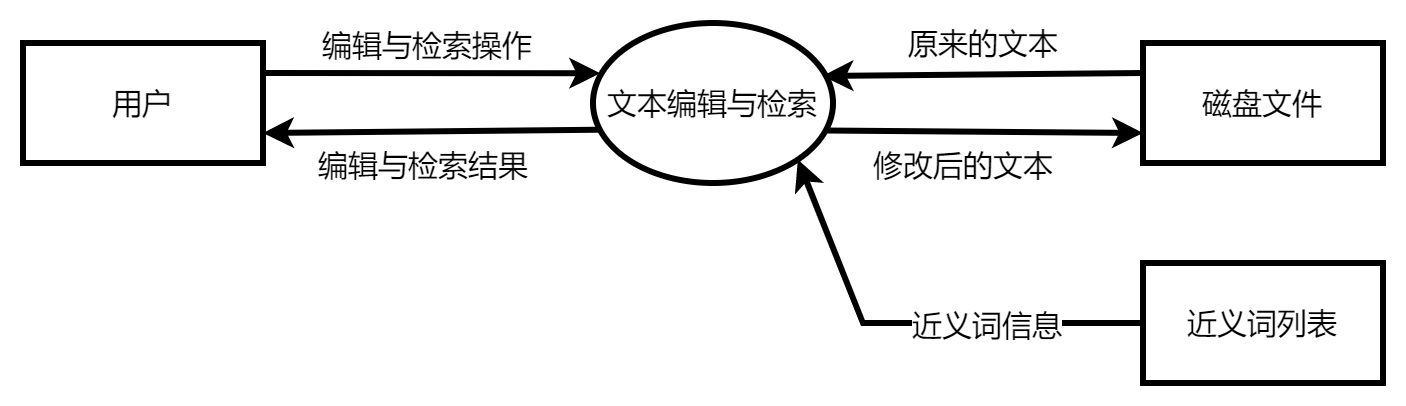
\includegraphics[width=\textwidth]{images/数据流图-第0层.png}
    \caption{数据流图-第0层}
\end{figure}

\begin{figure}[h]
    \centering
    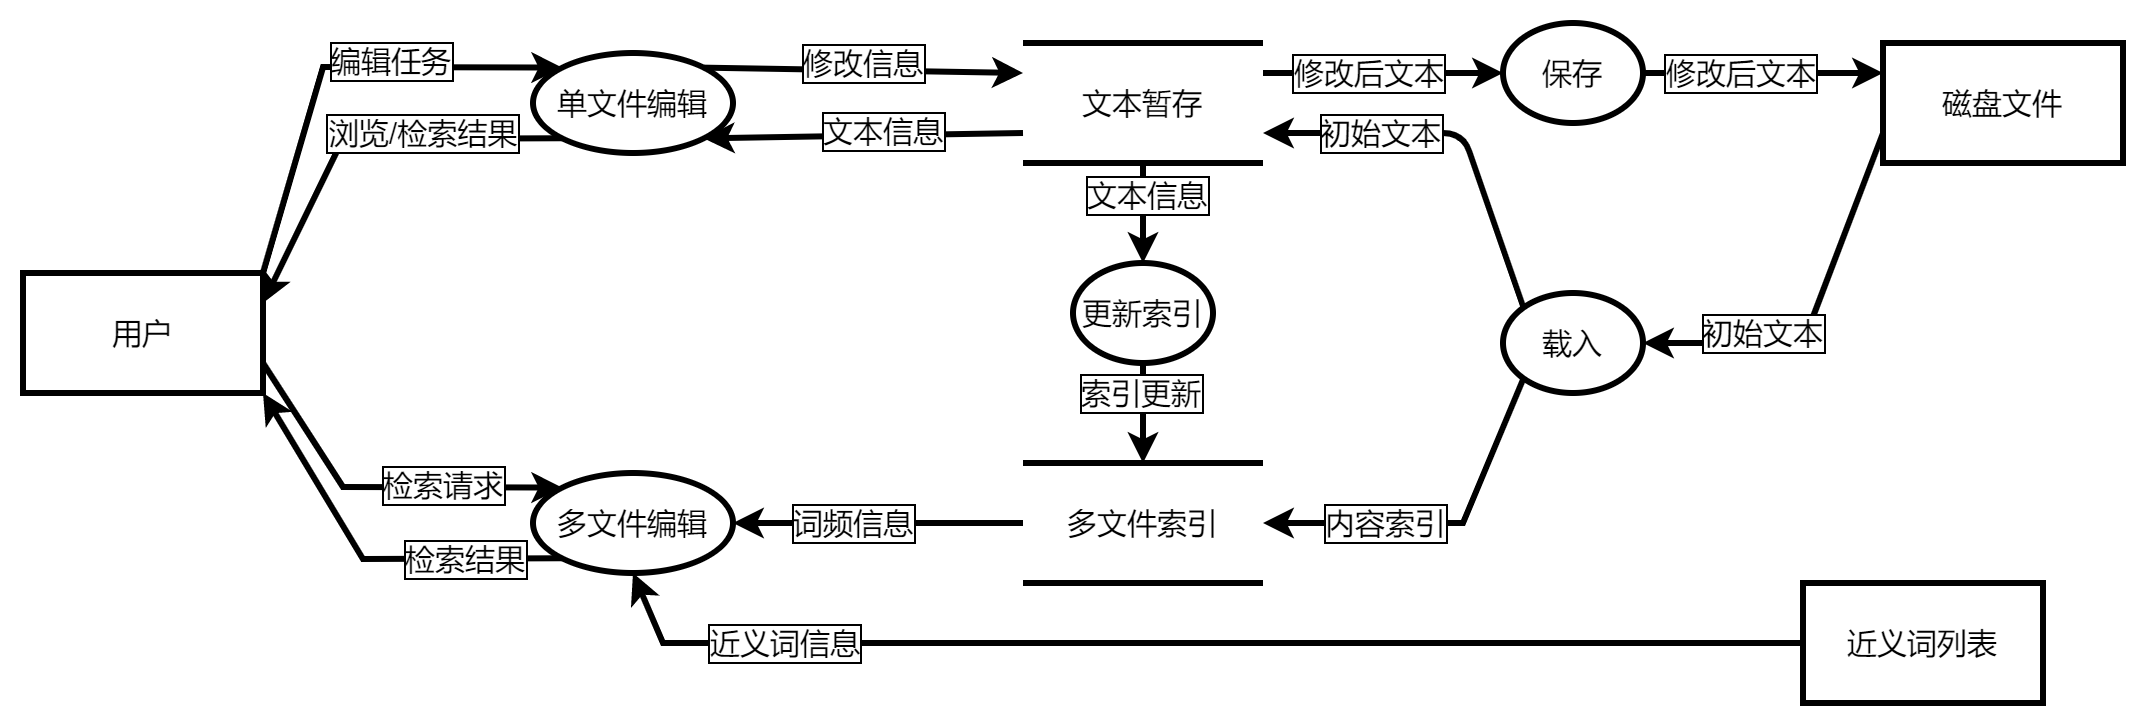
\includegraphics[width=\textwidth]{images/数据流图-第1层.png}
    \caption{数据流图-第1层}
\end{figure}

\begin{figure}[H]
    \centering
    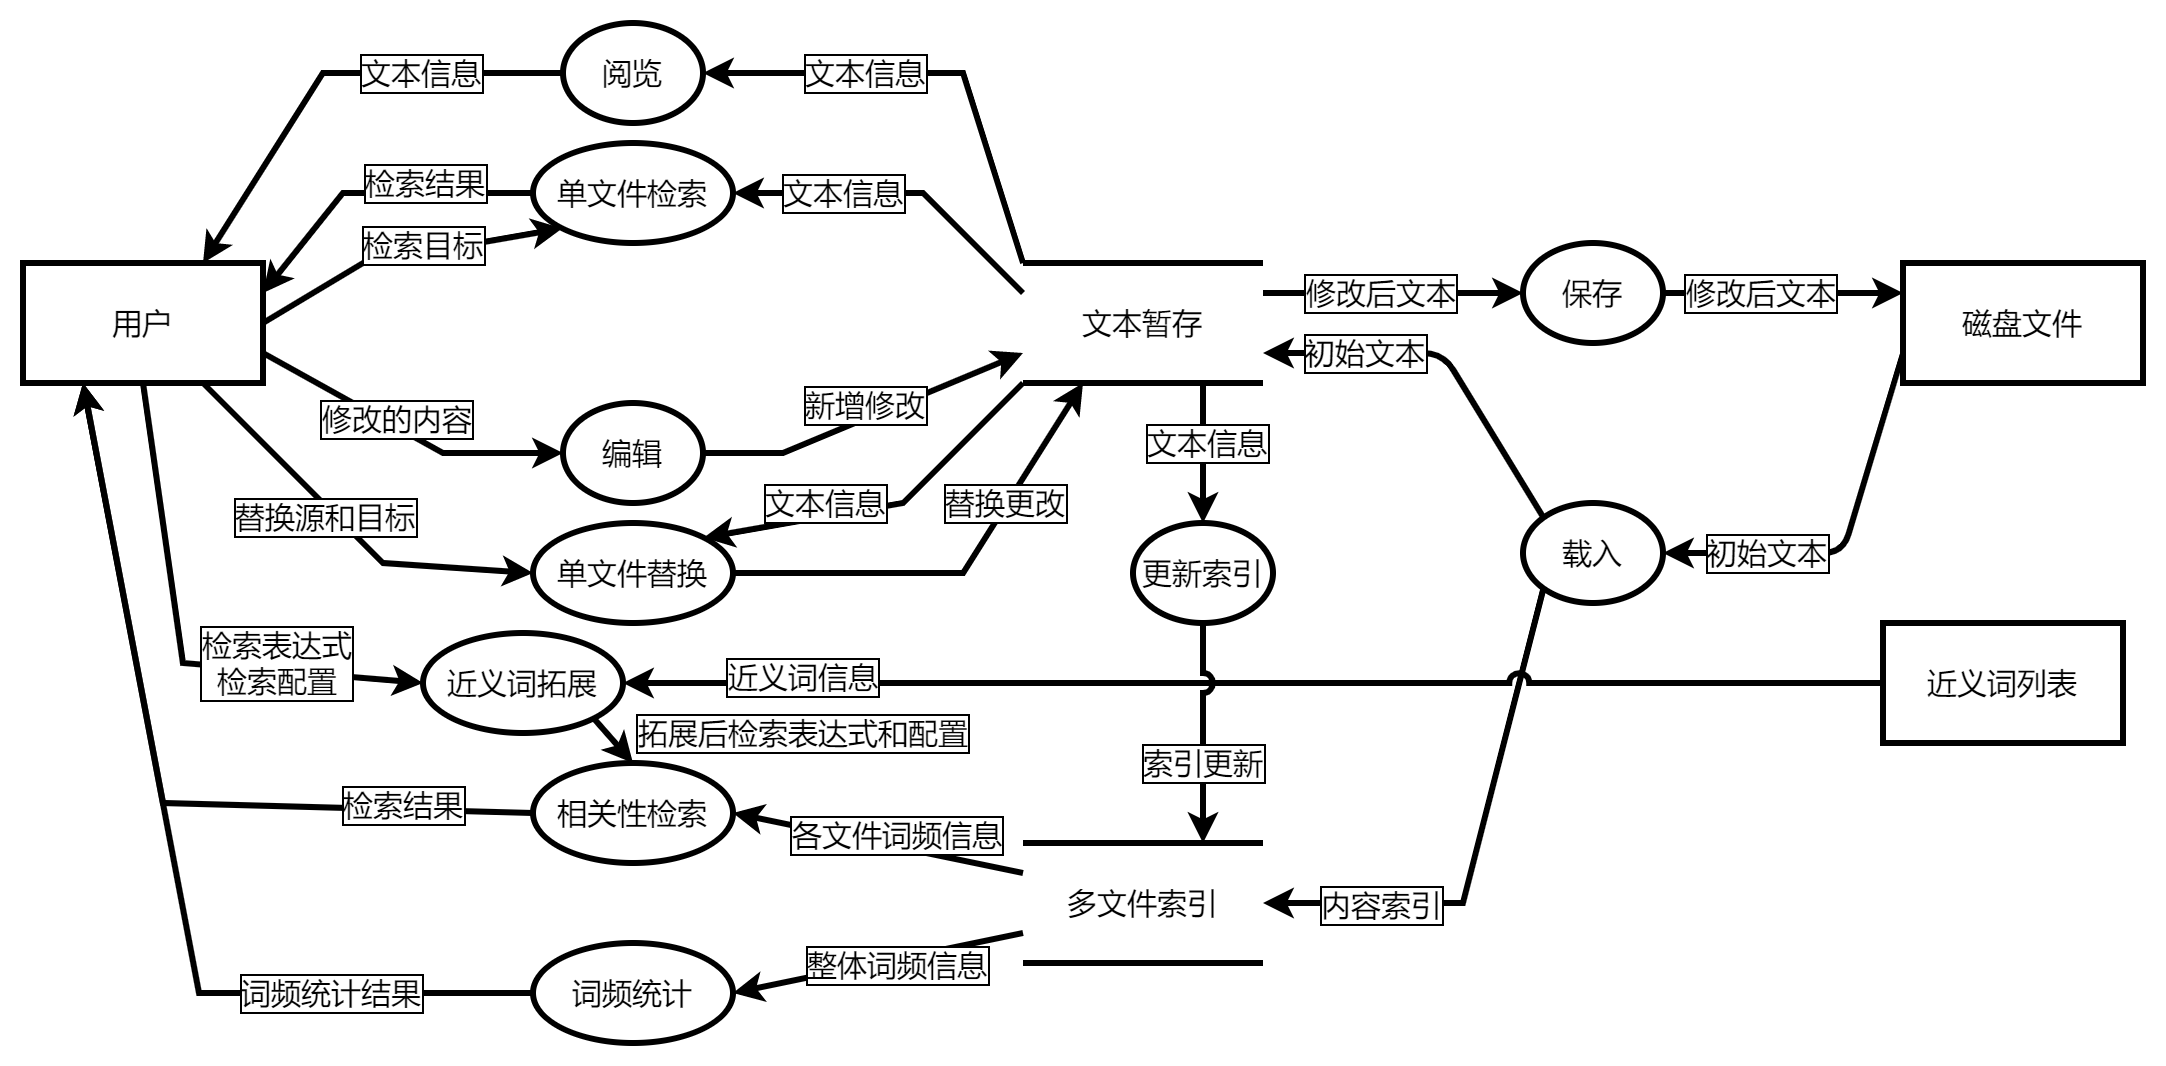
\includegraphics[width=\textwidth]{images/数据流图-第2层.png}
    \caption{数据流图-第2层}
\end{figure}

\clearpage

\subsection{使用iStar模型分析}

我使用iStar模型对需求进行分析。这里需求被分为多个结点,各结点参考左下角图示和以下的说明。

\begin{outline}
    \1 质量结点:表示非功能性需求
    \1 任务结点:表示功能性需求,连成三棵树
        \2 大字加粗的是树根,为总需求
        \2 最下方的叶子结点,为最基础的功能性需求
        \2 中间连接可用与、或的逻辑
\end{outline}

\begin{figure}[h]
    \centering
    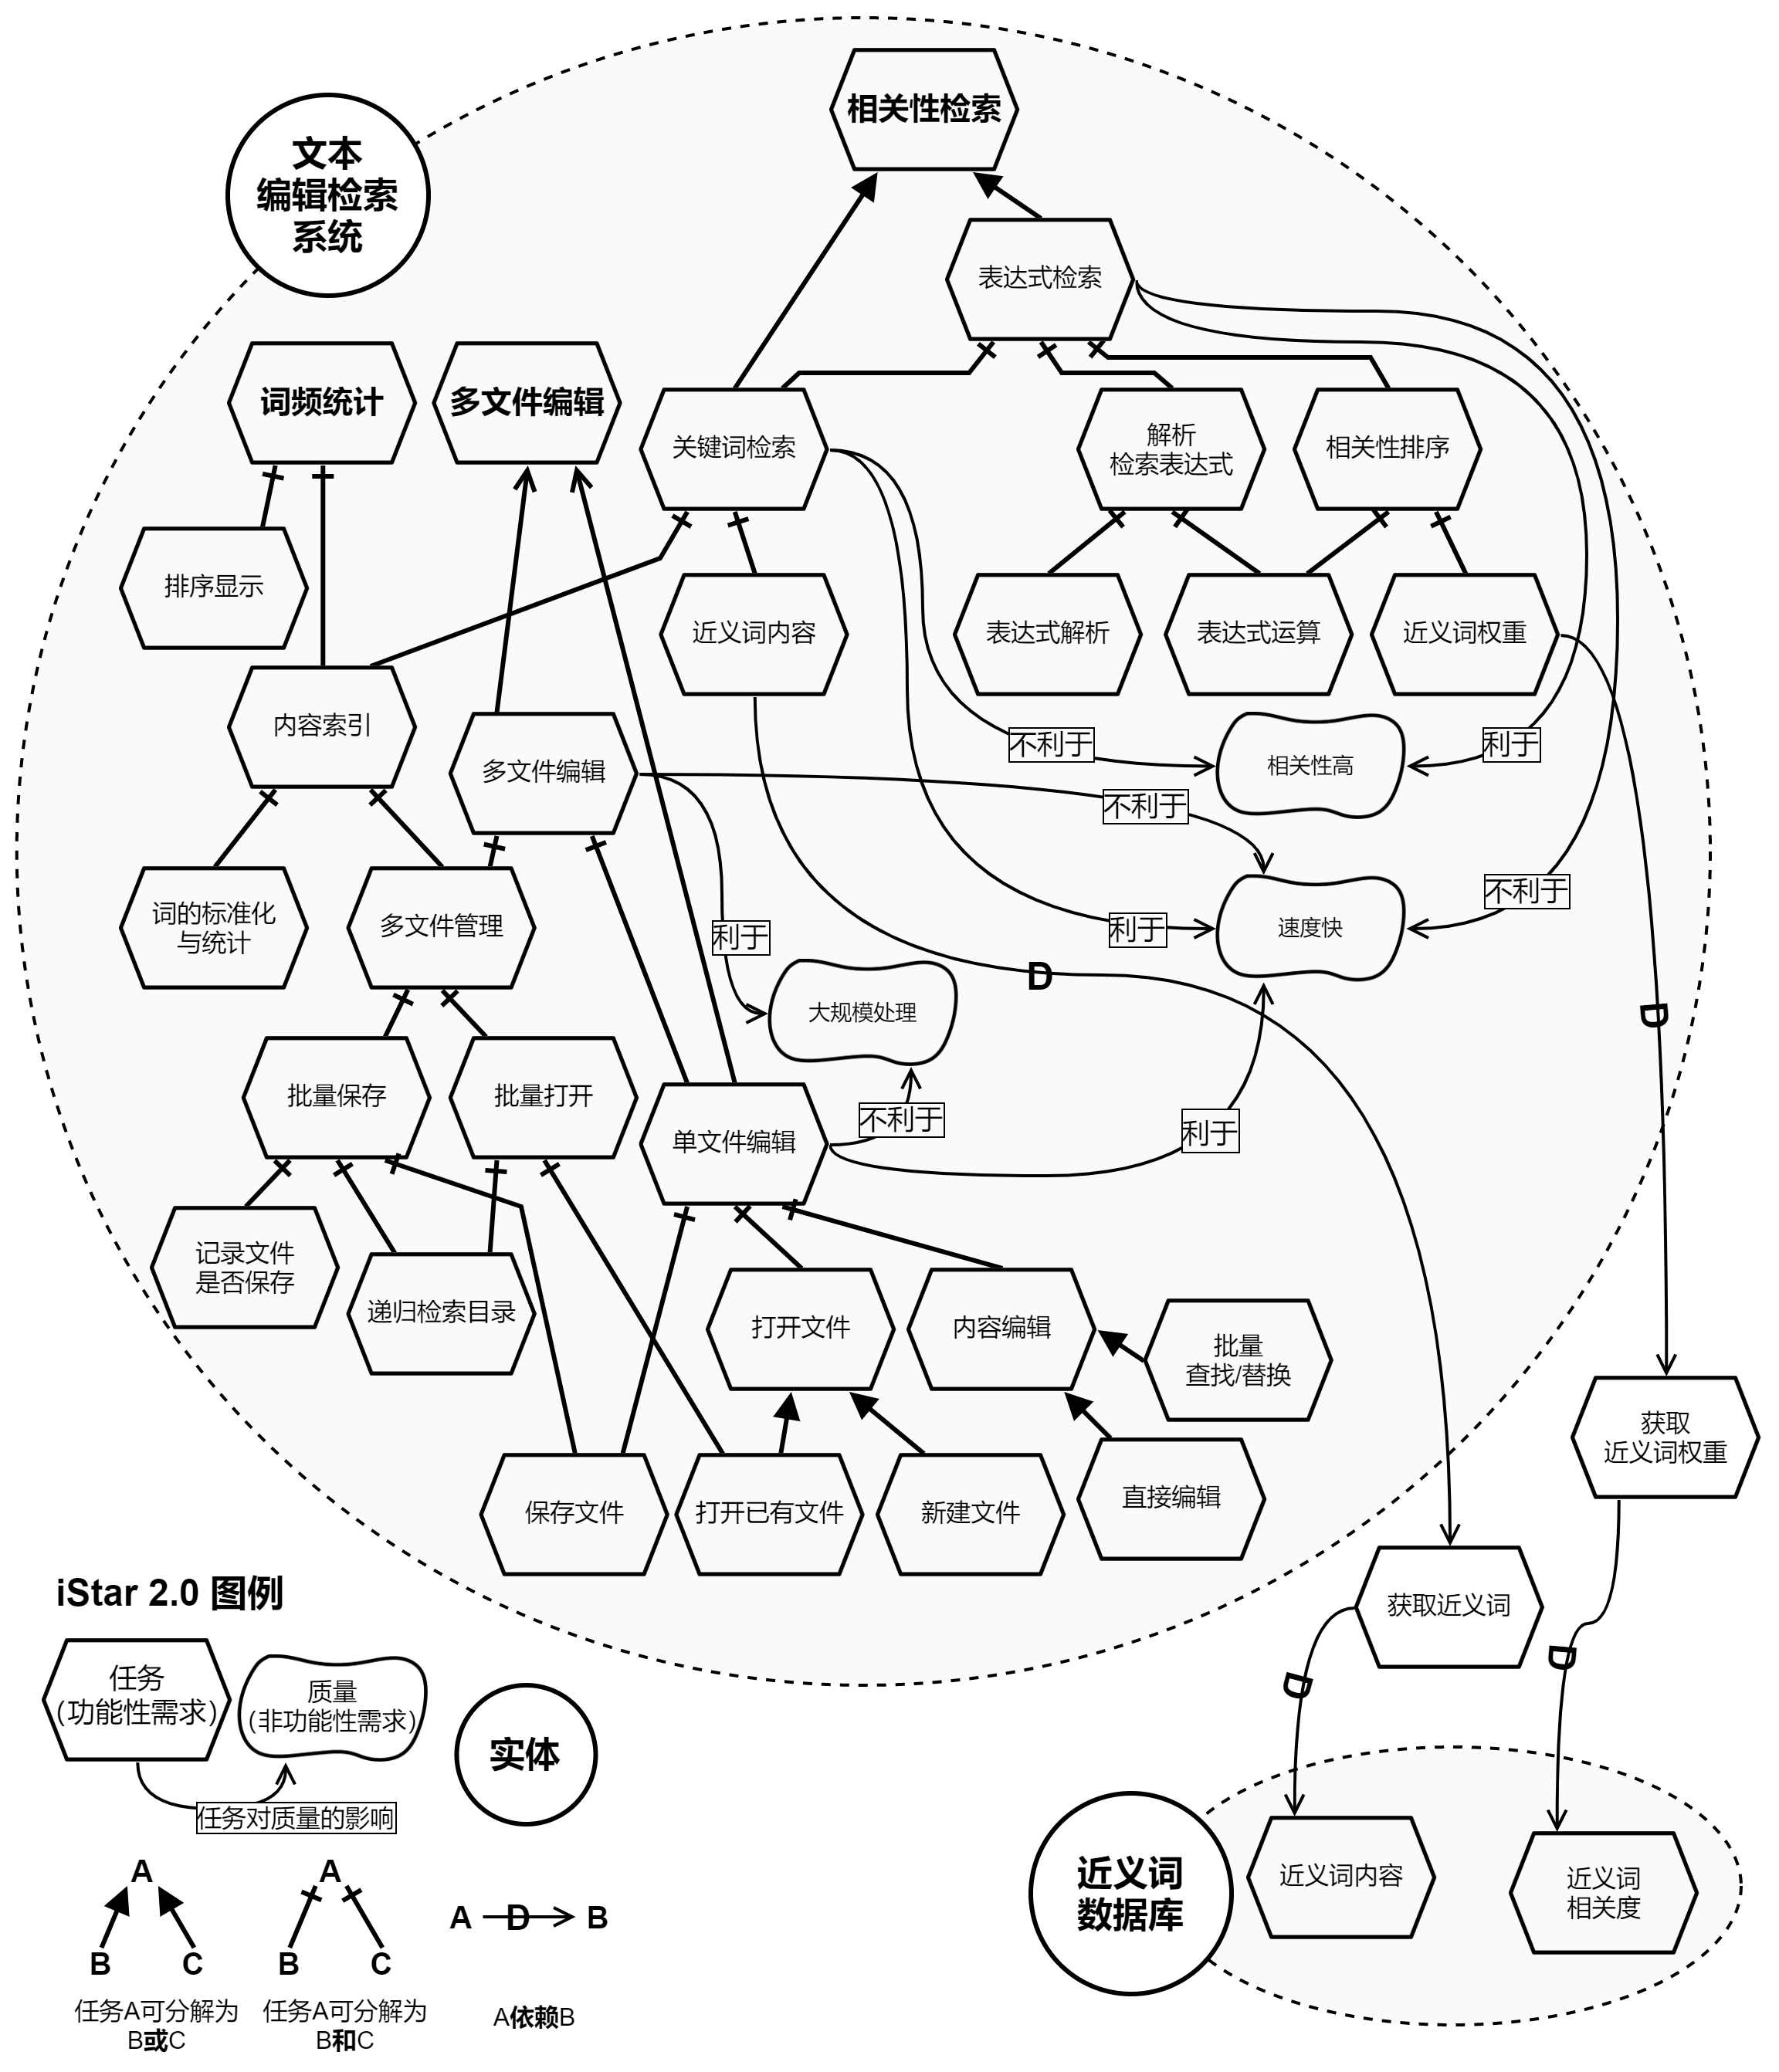
\includegraphics[width=\textwidth]{images/iStar.png}
    \caption{iStar模型图示}
\end{figure}

以上的iStar模型中展示了多种不同的方案,及其对非功能性需求带来的影响。考虑到速度减缓程度不大,且作为一款轻量型软件,通常只需要处理较少的数据。这里我均选择了牺牲速度,提高检索相关性、大规模处理多文件的方案。

而对于系统响应速度问题,我通过增加反馈信息的方式来提升用户对系统的了解情况。例如在为打开文件、保存文件、建立索引等操作时,都会在上方弹出提示。通过用提示丰富的方法,减缓了系统在处理大量数据时用时较长的弊端。

\subsection{需求分析结果}

通过上述两个方式进行需求分析,我总结分析出的大体的功能性需求如下:
\begin{outline}
    \1 文件管理
        \2 多文件结构化管理
        \2 批量打开、保存,记录文件保存状态
        \2 单文件打开、保存
    \1 文件编辑
        \2 单文件基础编辑
        \2 单文件搜索替换
    \1 多文件检索
        \2 表达式检索
        \2 可选地进行近义词拓展
        \2 可选择查看任意数量的结果
    \1 词频统计
        \2 可选择查看任意数量的结果
\end{outline}

\part{原型设计说明}
\section{一代原型设计}
一代原型设计采用抛弃型原型,使用绘图工具绘制矢量图。其价值主要在于确定系统的主要功能、界面效果。由于没有具体设计动态的人机交互方式,人机交互相关的部分我们主要在二代原型设计中说明。

一代原型设计时并没有进行好详细的需求分析,为此存在一些问题,这些问题在后续进行了改进。

以下为一代原型设计,左边为图形界面预览,右边是对对应界面功能的说明。

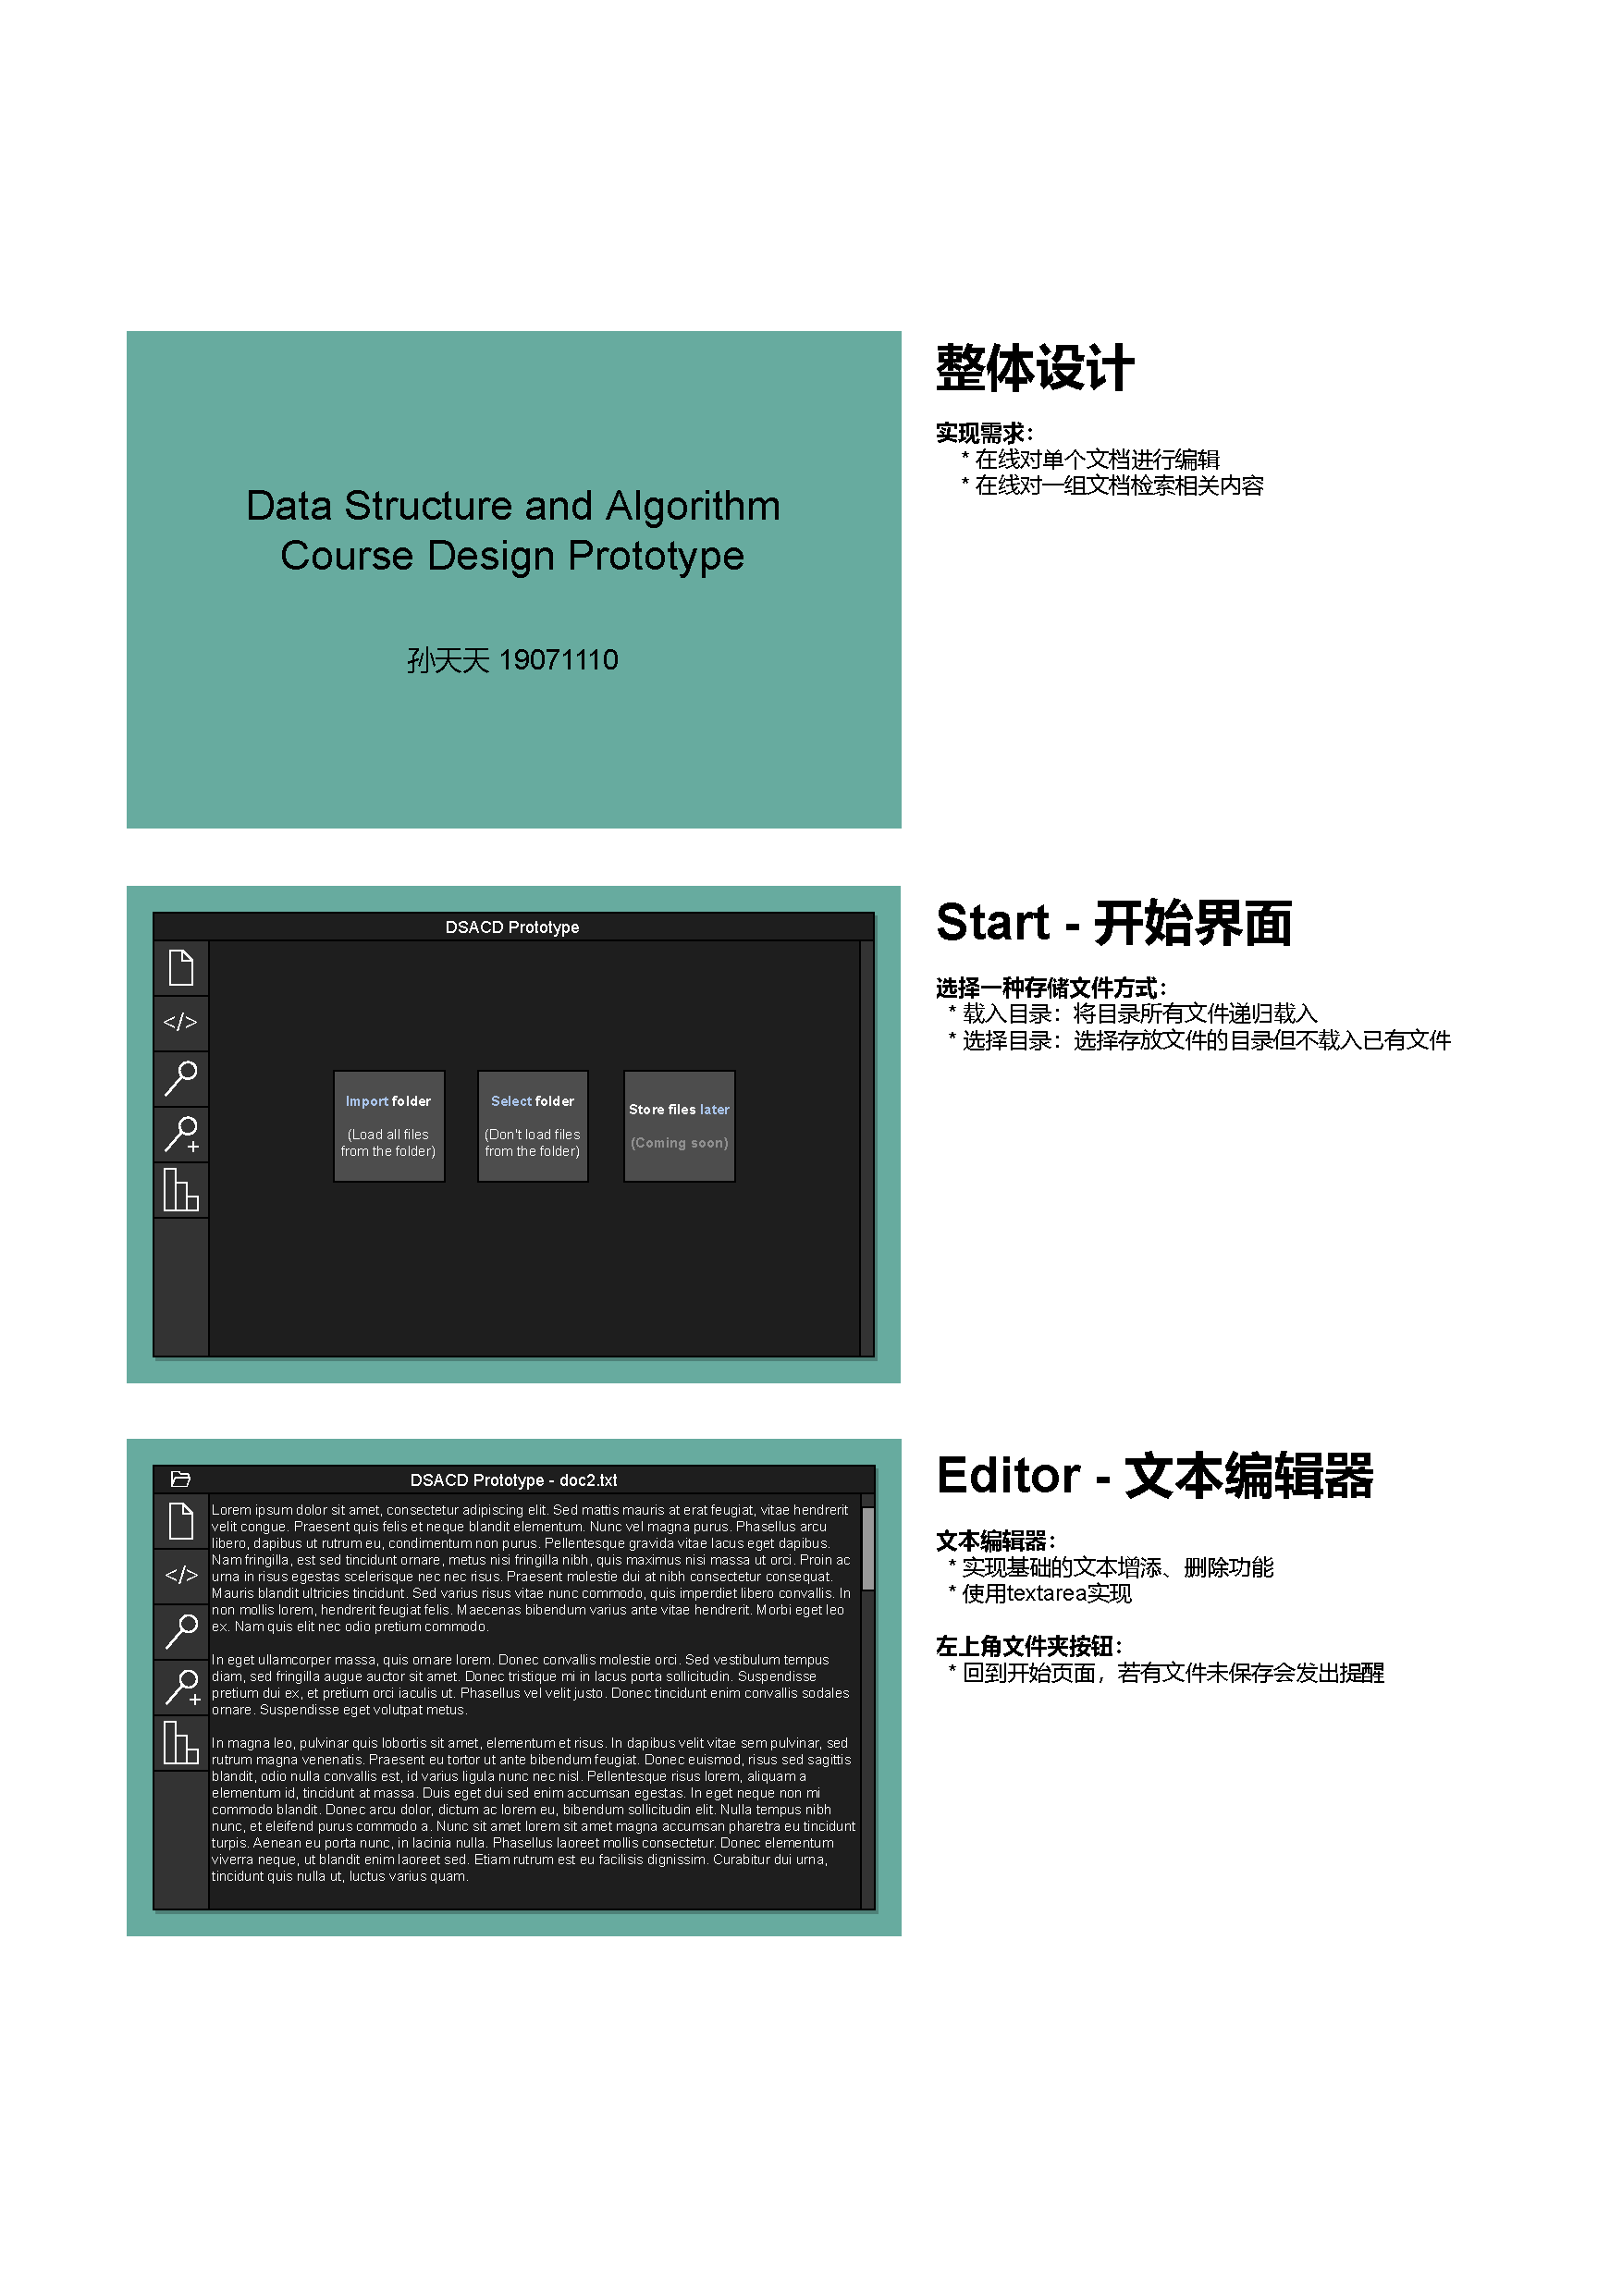
\includepdf[pages=-,pagecommand={},width=1.5\textwidth]{prototypev1.pdf}

\section{二代原型设计}
二代原型设计采用进化式原型,选择使用web前端代码开发(Vue+Ant Design For Vue组件库)的形式。
但由于技术难度和工作量的原因,仍然只实现了与人机交互相关度较高的部分。为实现的部分会在下面说明。

二代原型采用分层设计框架。具体如下:

\subsection{功能层}
功能层即功能性需求,与需求分析中总结的主要功能性需求一致。包括以下四个主要的部分:
\begin{outline}
    \1 文件管理
    \1 文件编辑
    \1 多文件检索
    \1 词频统计
\end{outline}

\subsection{架构层}
\subsubsection{整体布局}
架构层中,我首先将用户界面可切换部分分为侧栏和编辑器栏两部分。此外还有页眉、页脚和菜单切换三个固定的部分。
侧栏和编辑器栏中间有一个自动滑动模块,用户可以自由分配两个栏的空间。

\begin{figure}[h]
    \centering
    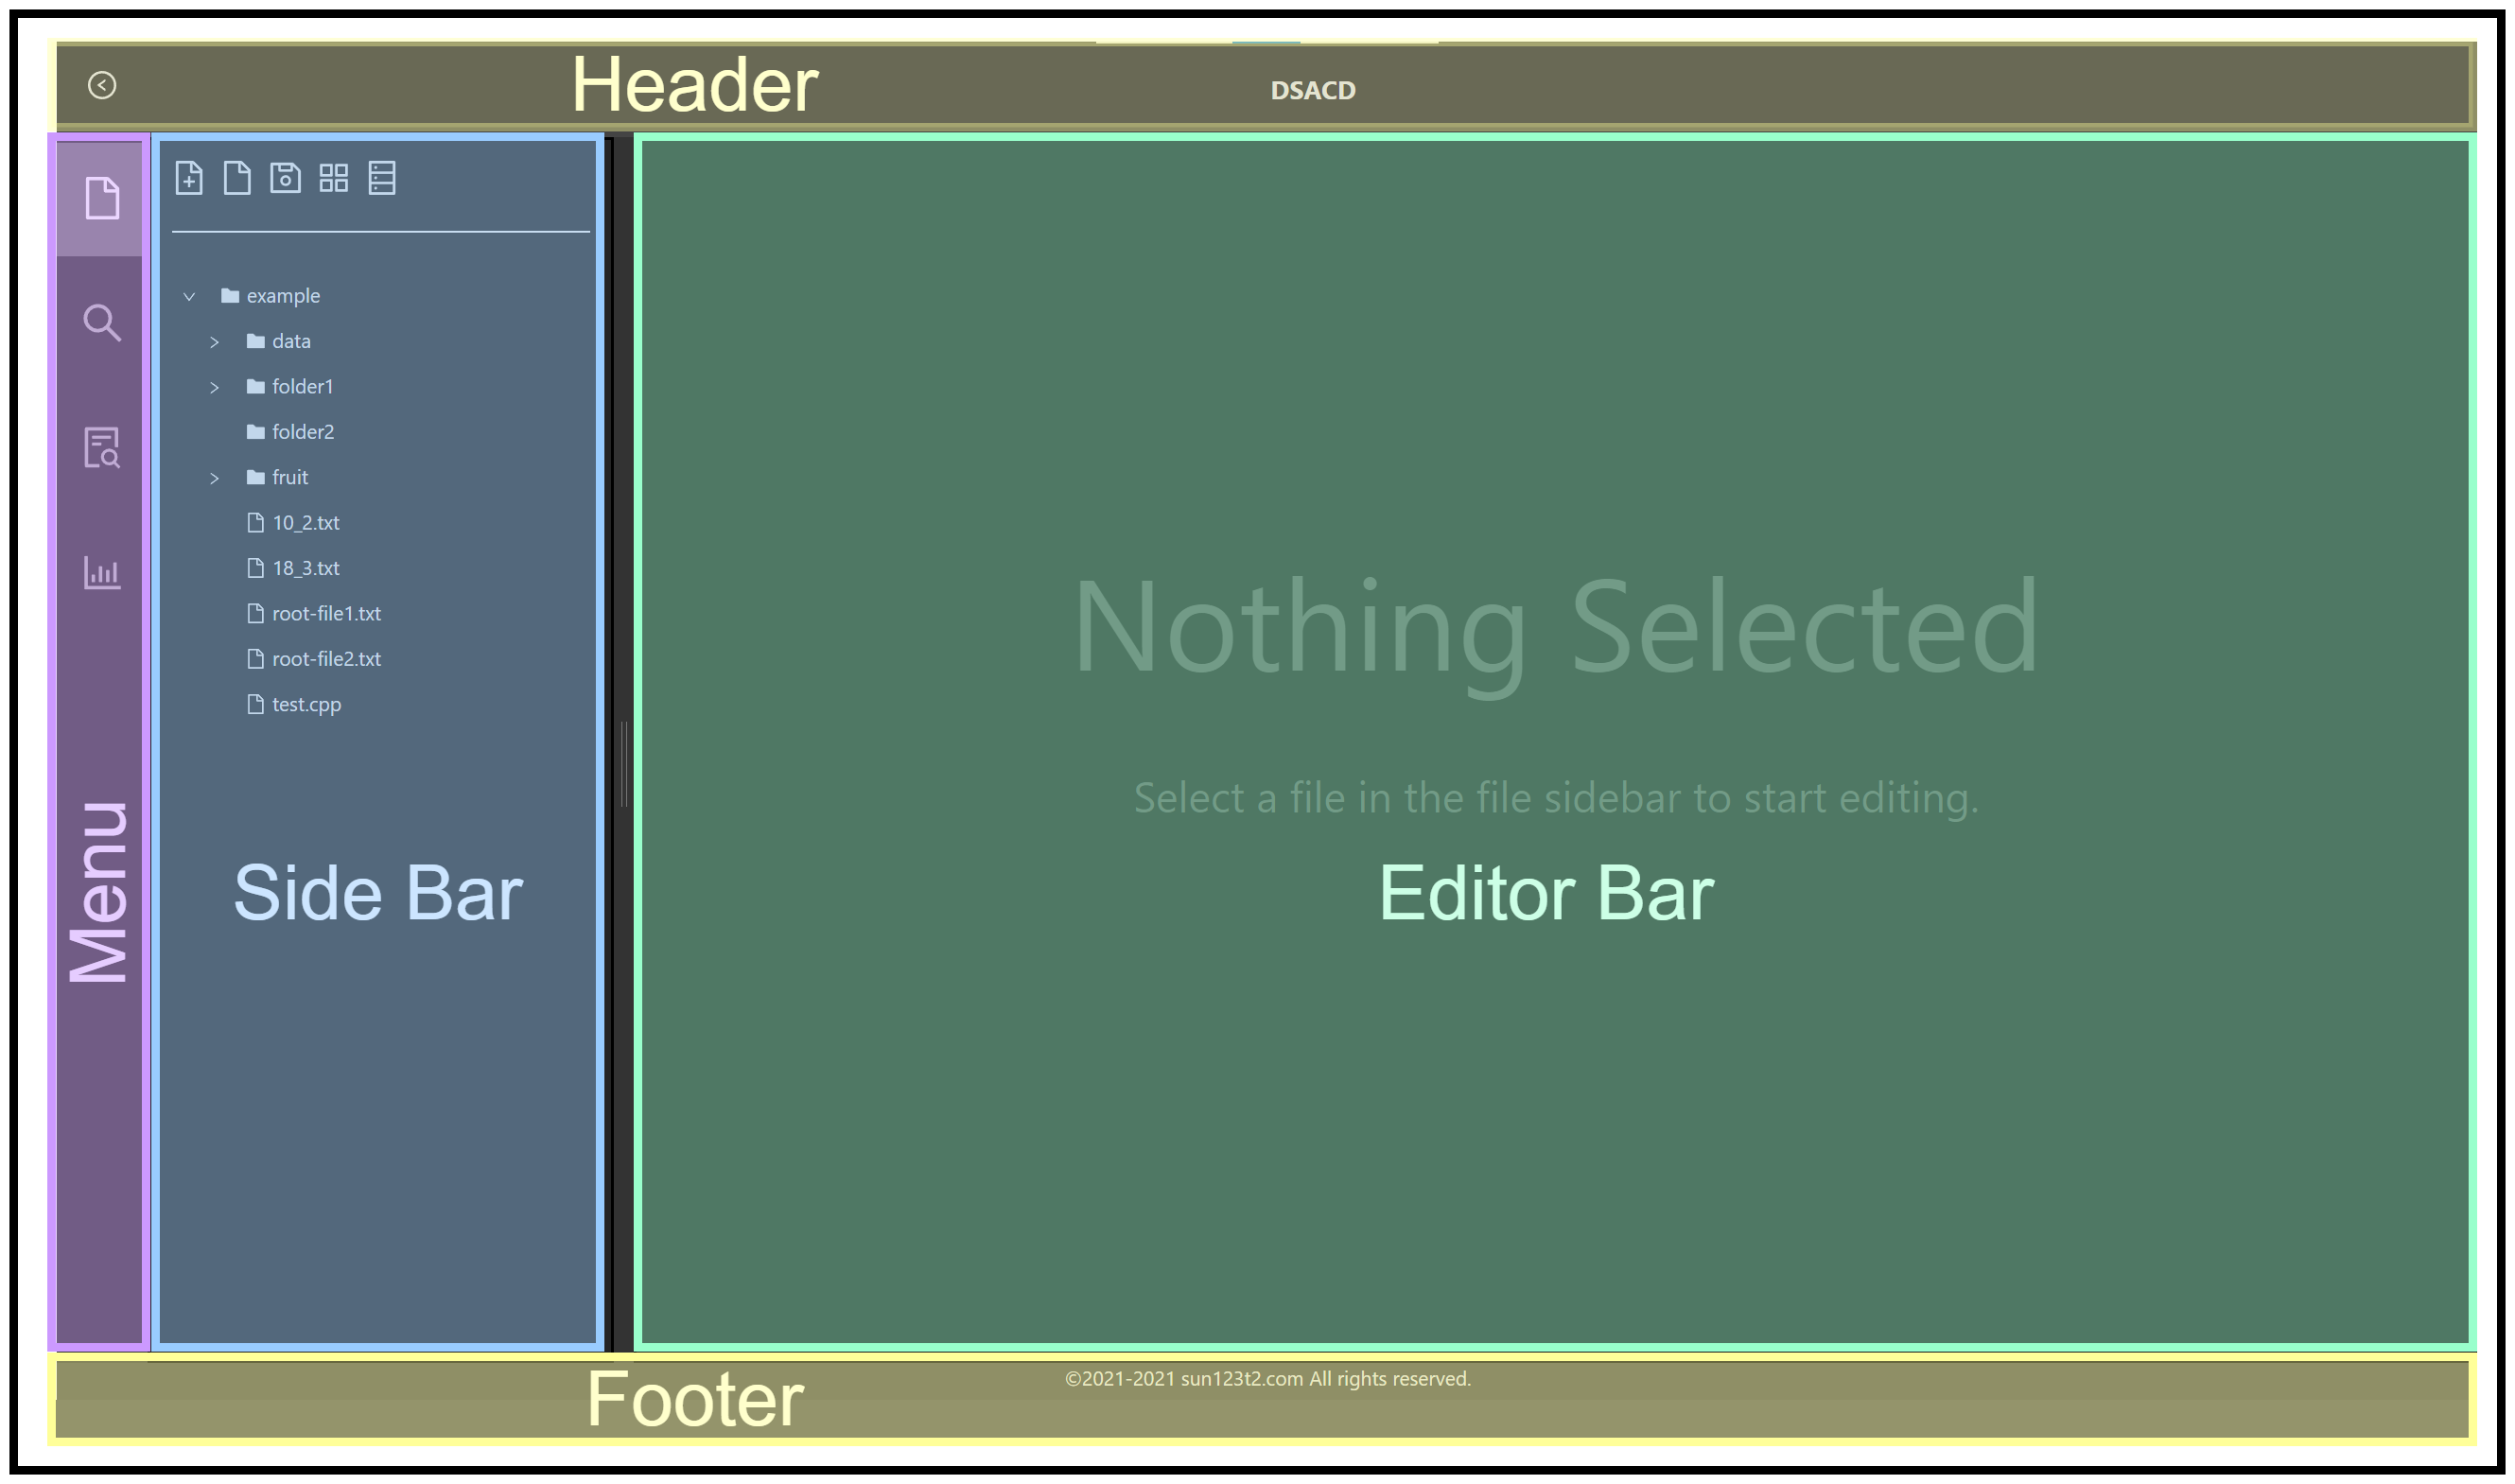
\includegraphics[width=\textwidth]{images/dsacd-screenshot-layout-.drawio.png}
    \caption{整体布局}
\end{figure}

\clearpage

\subsubsection{内容模块划分}
根据功能,我为侧栏和编辑器栏各设计了几个功能模块。

\paragraph{侧栏模块} 侧栏包含:文件管理、单文件检索替换、相关性搜索和词频统计,这四个模块。

它们分别对应功能层中的文件管理、文件编辑(检索替换)、多文件检索、词频统计四个功能需求。

用户可以在最左侧的菜单栏随时切换侧栏。此外,侧栏也可以收起,既不展示任何一个侧栏

\paragraph{编辑器栏模块} 编辑器栏包括:开始界面、编辑器、目录预览器和暂无内容提示,这四个模块。

其中第一个开始界面为管理文件中载入的部分服务。其余三个模块对应选中文件、选中目录和未选中三种状态,其中核心是编辑器模块,实现了文件编辑(直接编辑)的功能性需求,其他几个模块用于处理其他情况。

编辑器栏会根据是否已经选择目标目录和当前选中的文件或目录自动切换。

\begin{figure}[h]
    \centering
    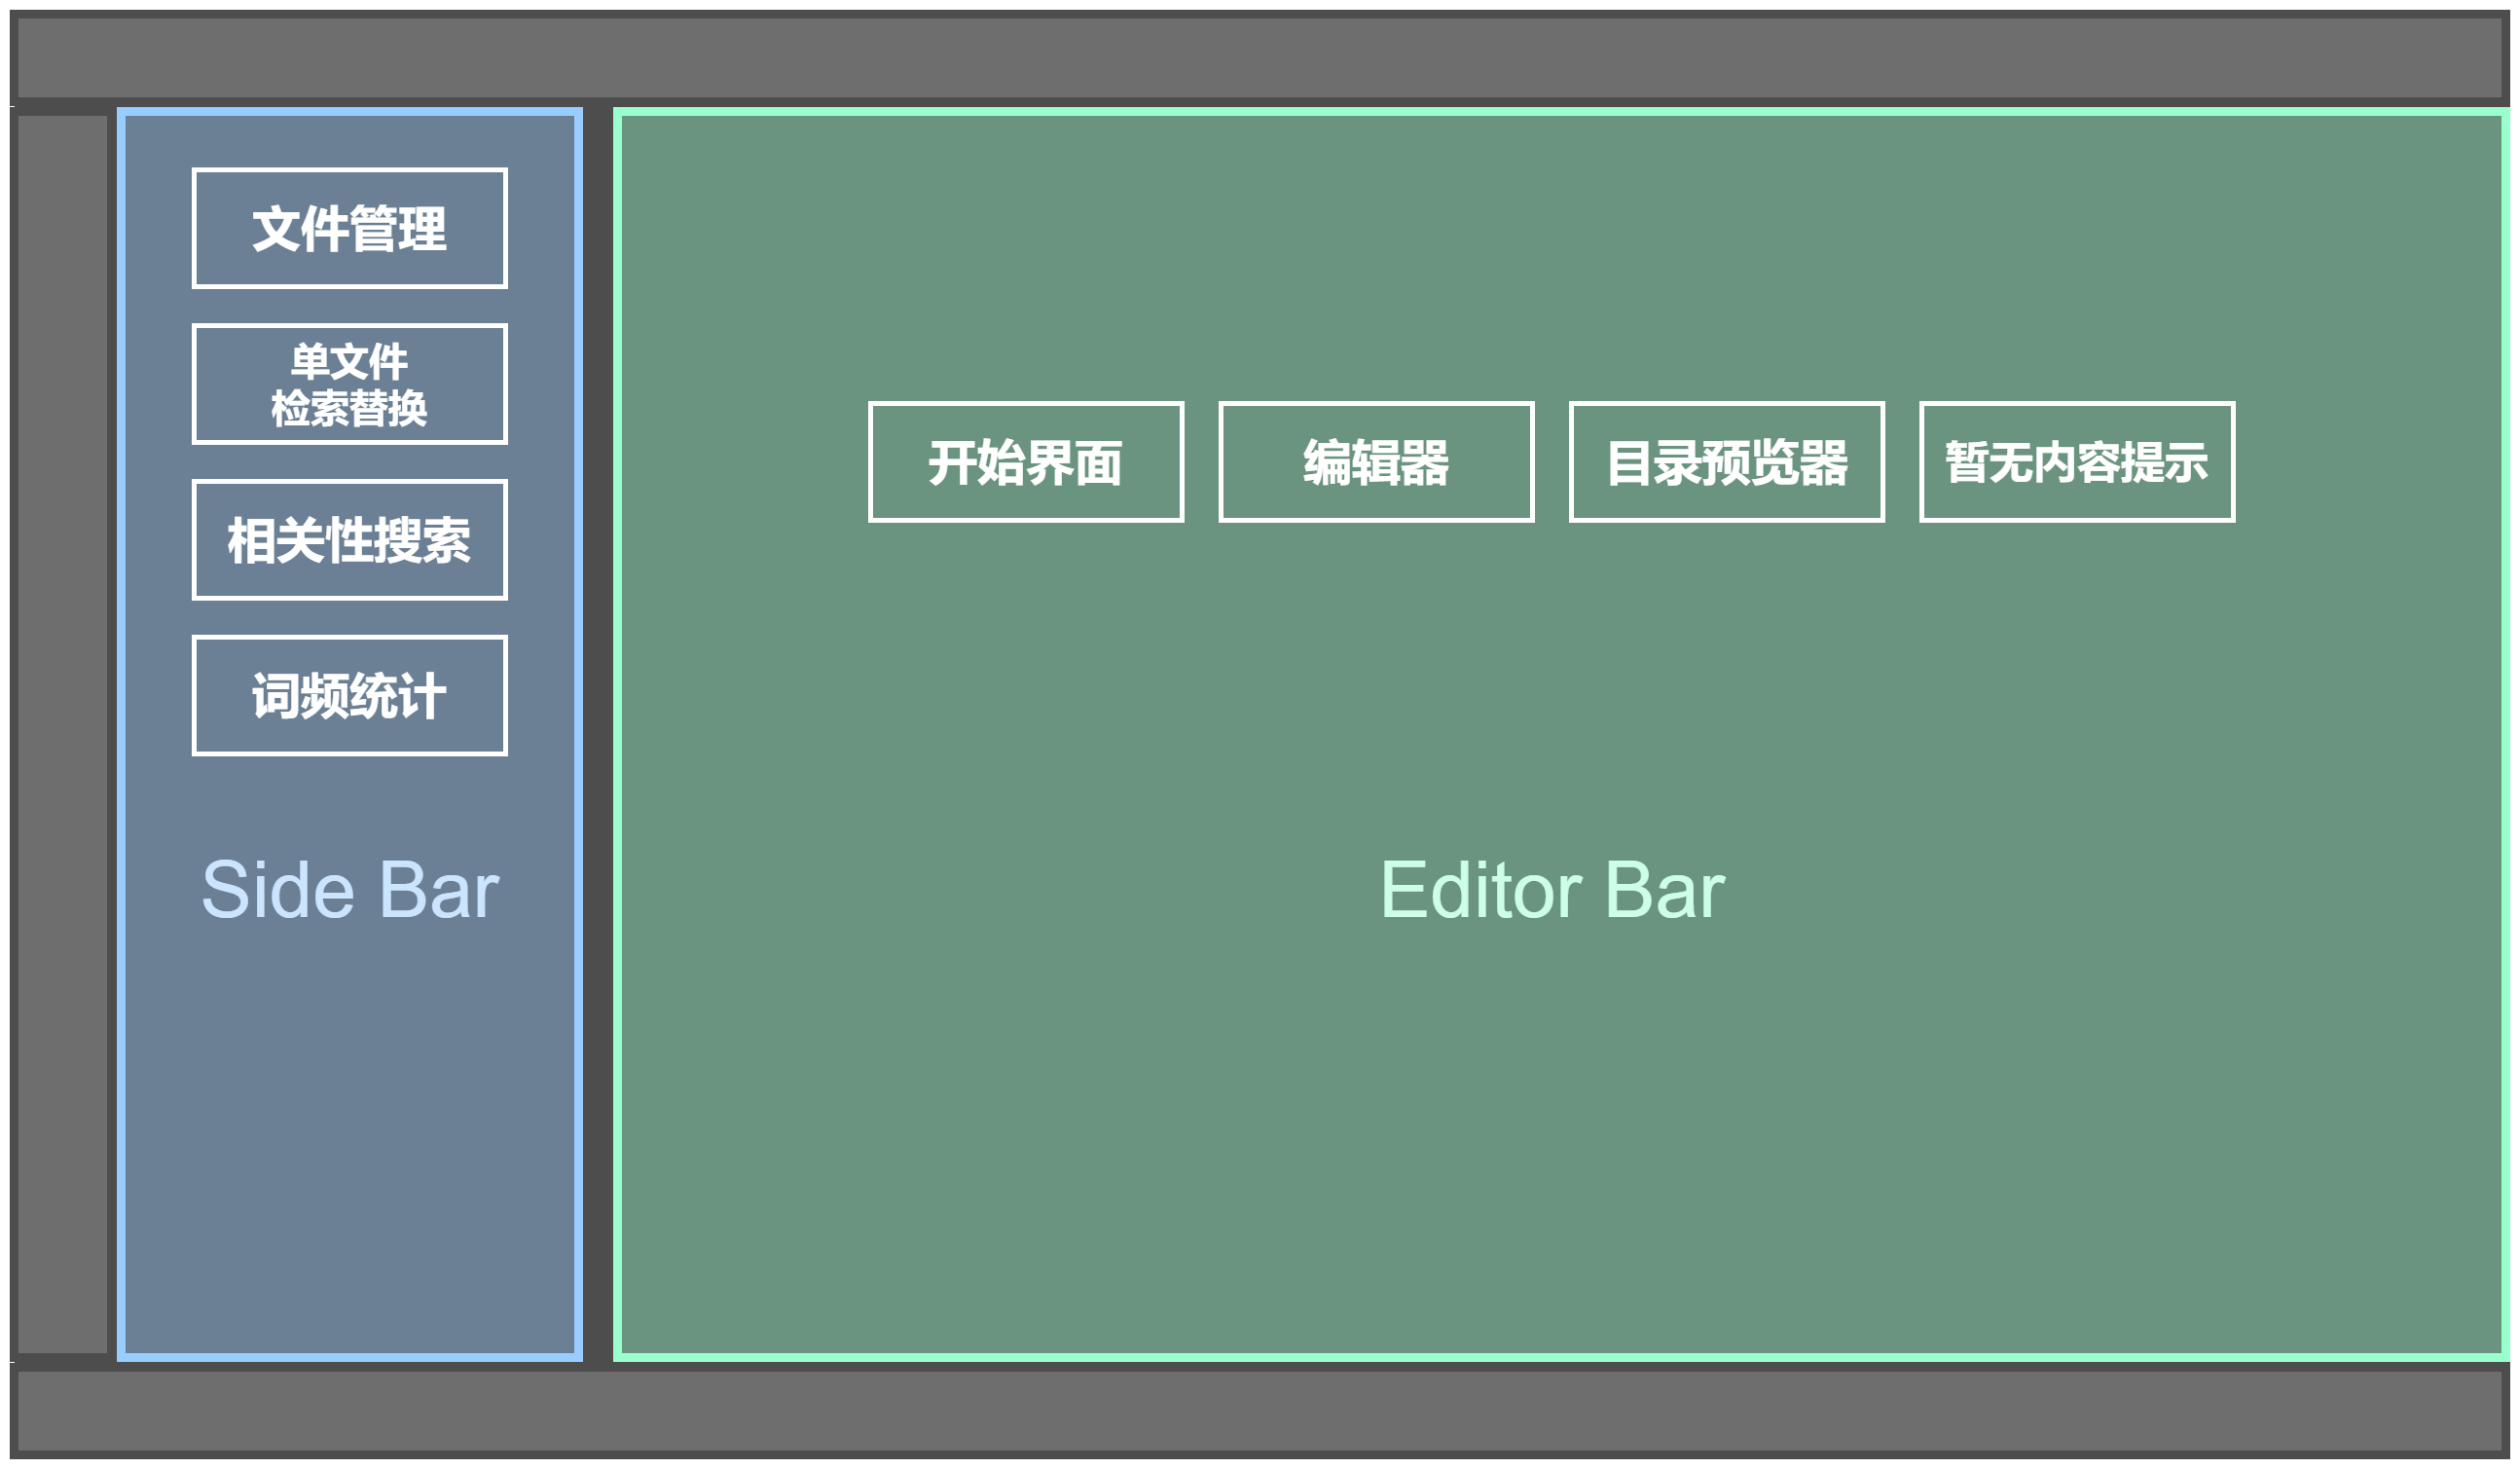
\includegraphics[width=\textwidth]{images/dsacd-screenshot-modules.drawio.png}
    \caption{两栏的各四个模块}
\end{figure}

\subsection{导航层}

架构层中将界面分为了两个可切换部分:侧栏和编辑器栏,而每个部分又各有4各模块。导航层则重点说明这两部分各自内部模块间的连接关系、两个部分之间的联动关系。

\paragraph{启动约束}

系统启动后,两部分的模块选择状态如图中黑色箭头所示。Start表示系统启动,首先侧栏收起,编辑器栏进入开始界面。这个时候用户必须选择目标目录,无法更改模块。

当用户选择目标目录后,界面顺着黑色箭头分别来到文件管理、暂无内容提示。随后启动约束解除,用户可以按照自己的意愿按照白色箭头任意切换。

\clearpage

\begin{figure}[h]
    \centering
    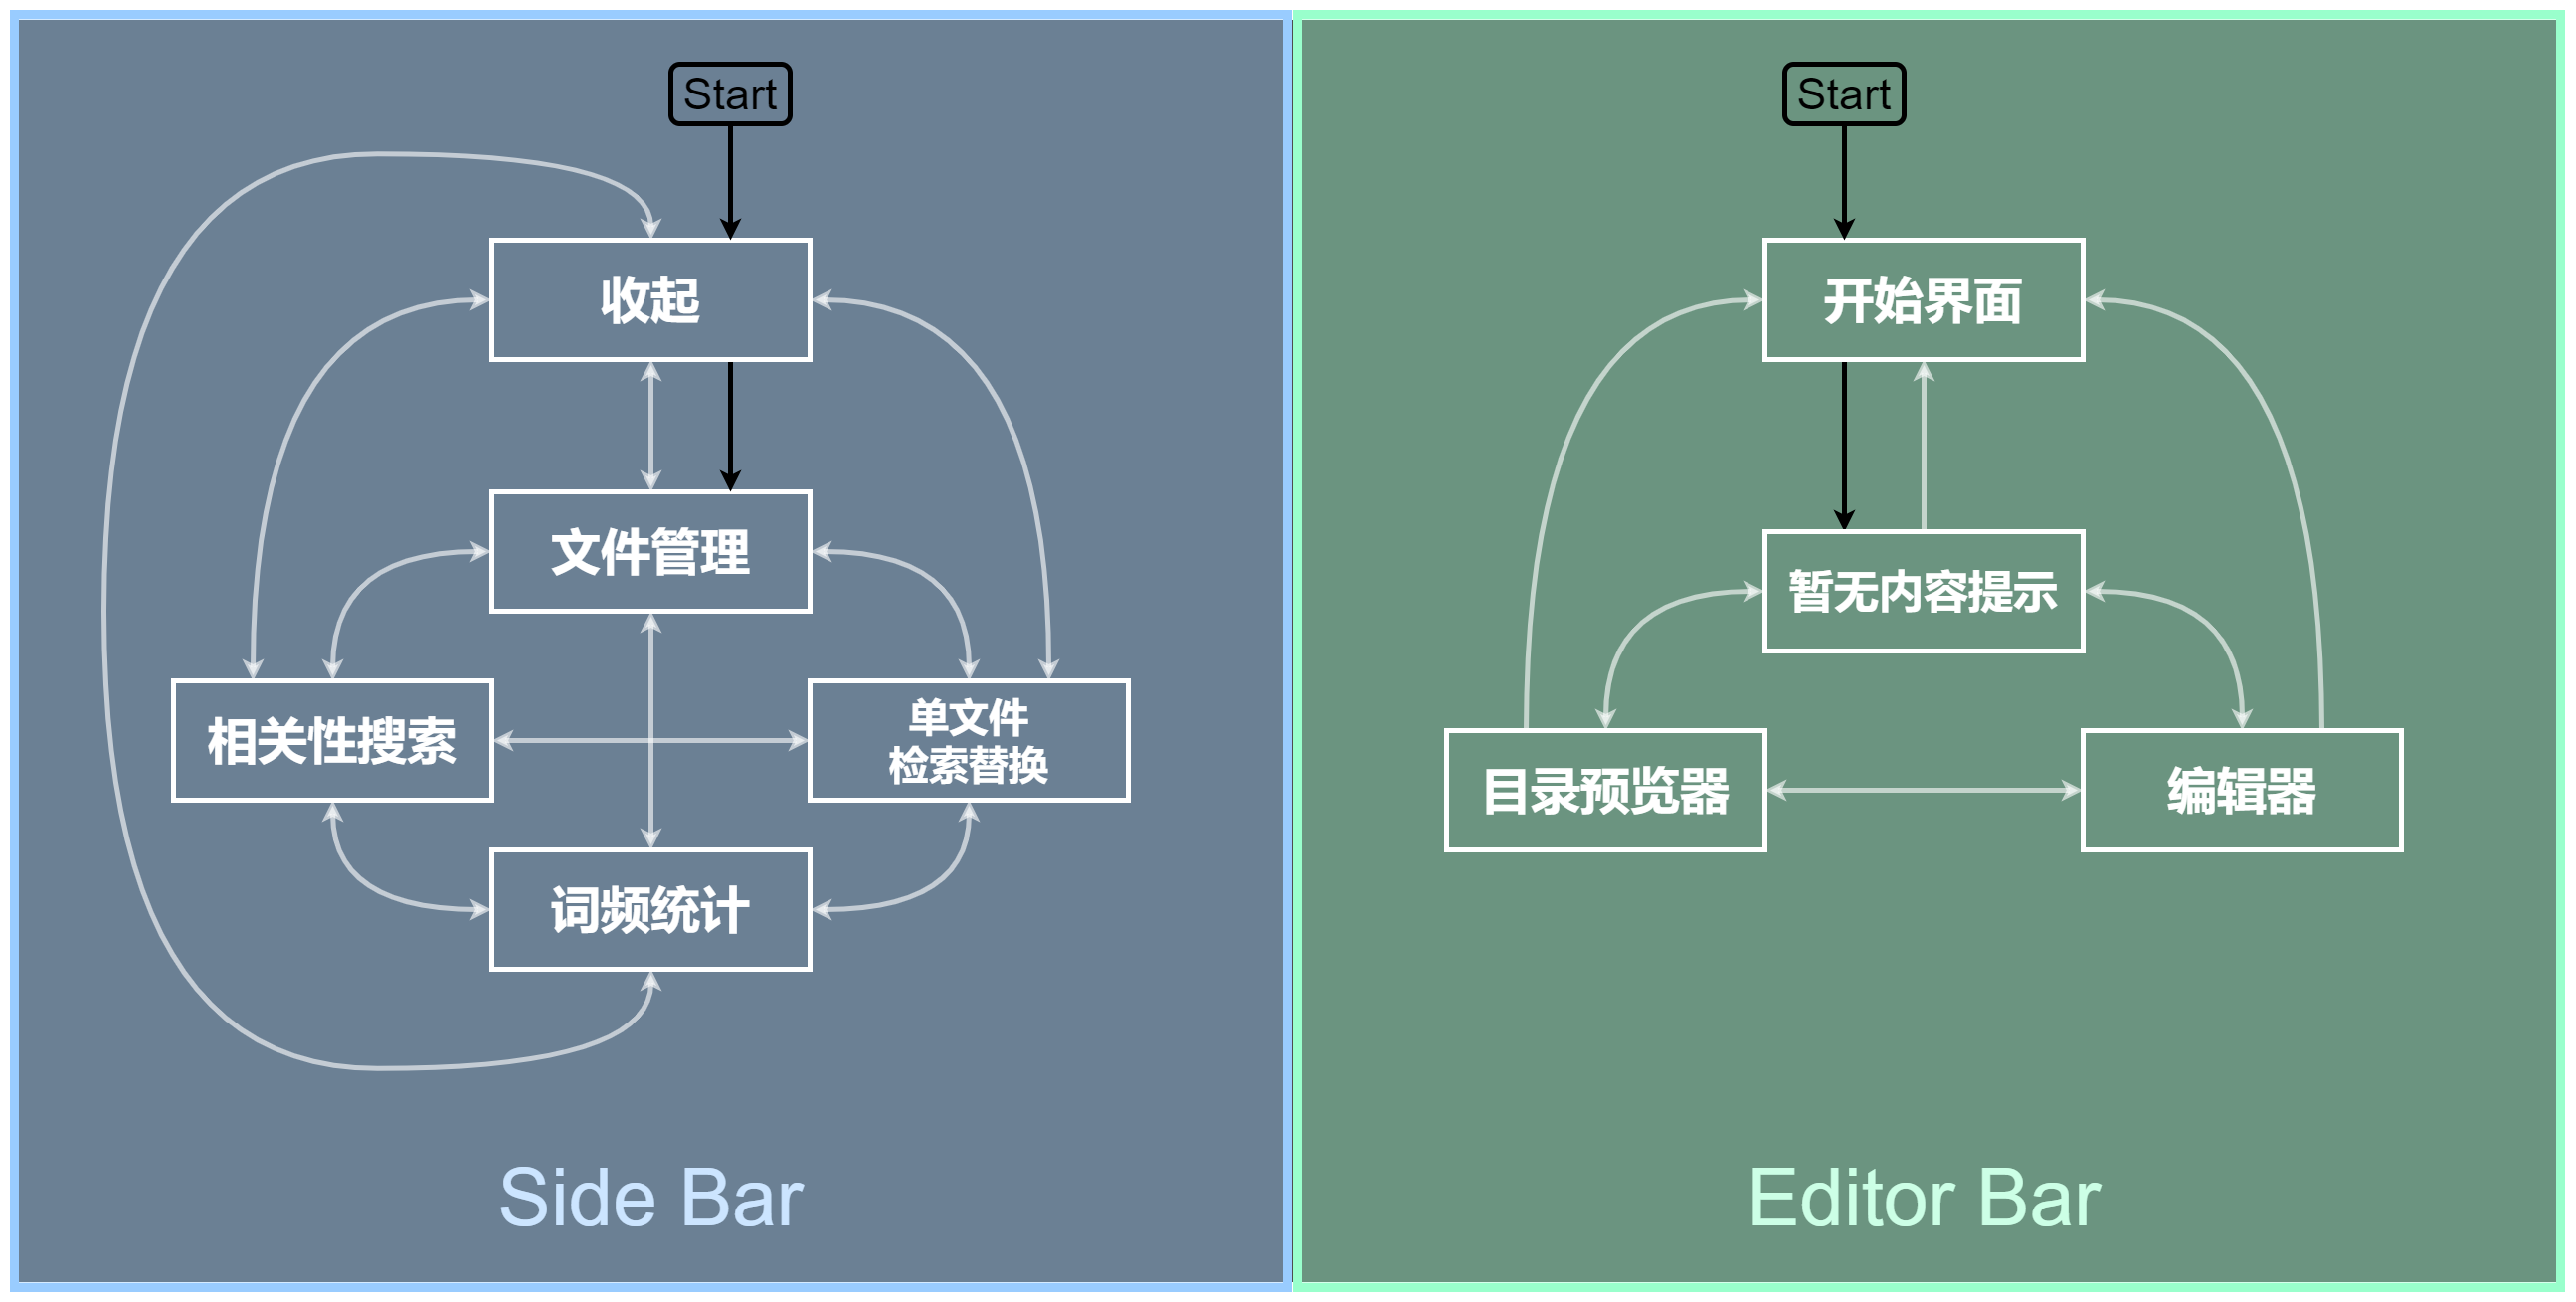
\includegraphics[width=\textwidth]{images/dsacd-screenshot-switch.drawio.png}
    \caption{各模块切换}
\end{figure}

\paragraph{侧栏部分}
侧栏部分的跳转模式基本上是全连接模式。除非在启动约束下,用户可以随意选择自己需要使用的功能。这一点与任意时刻可以自由选择功能进行编辑的需求相符。

侧栏左侧的菜单栏会时刻高亮当前选中的模块,以此提示用户自己当前的位置;同时,未高亮的部分可以提示用户其他可用的功能。特别地,收起时,菜单栏不会高亮任何一个图标。

\begin{figure}[h]
    \centering
    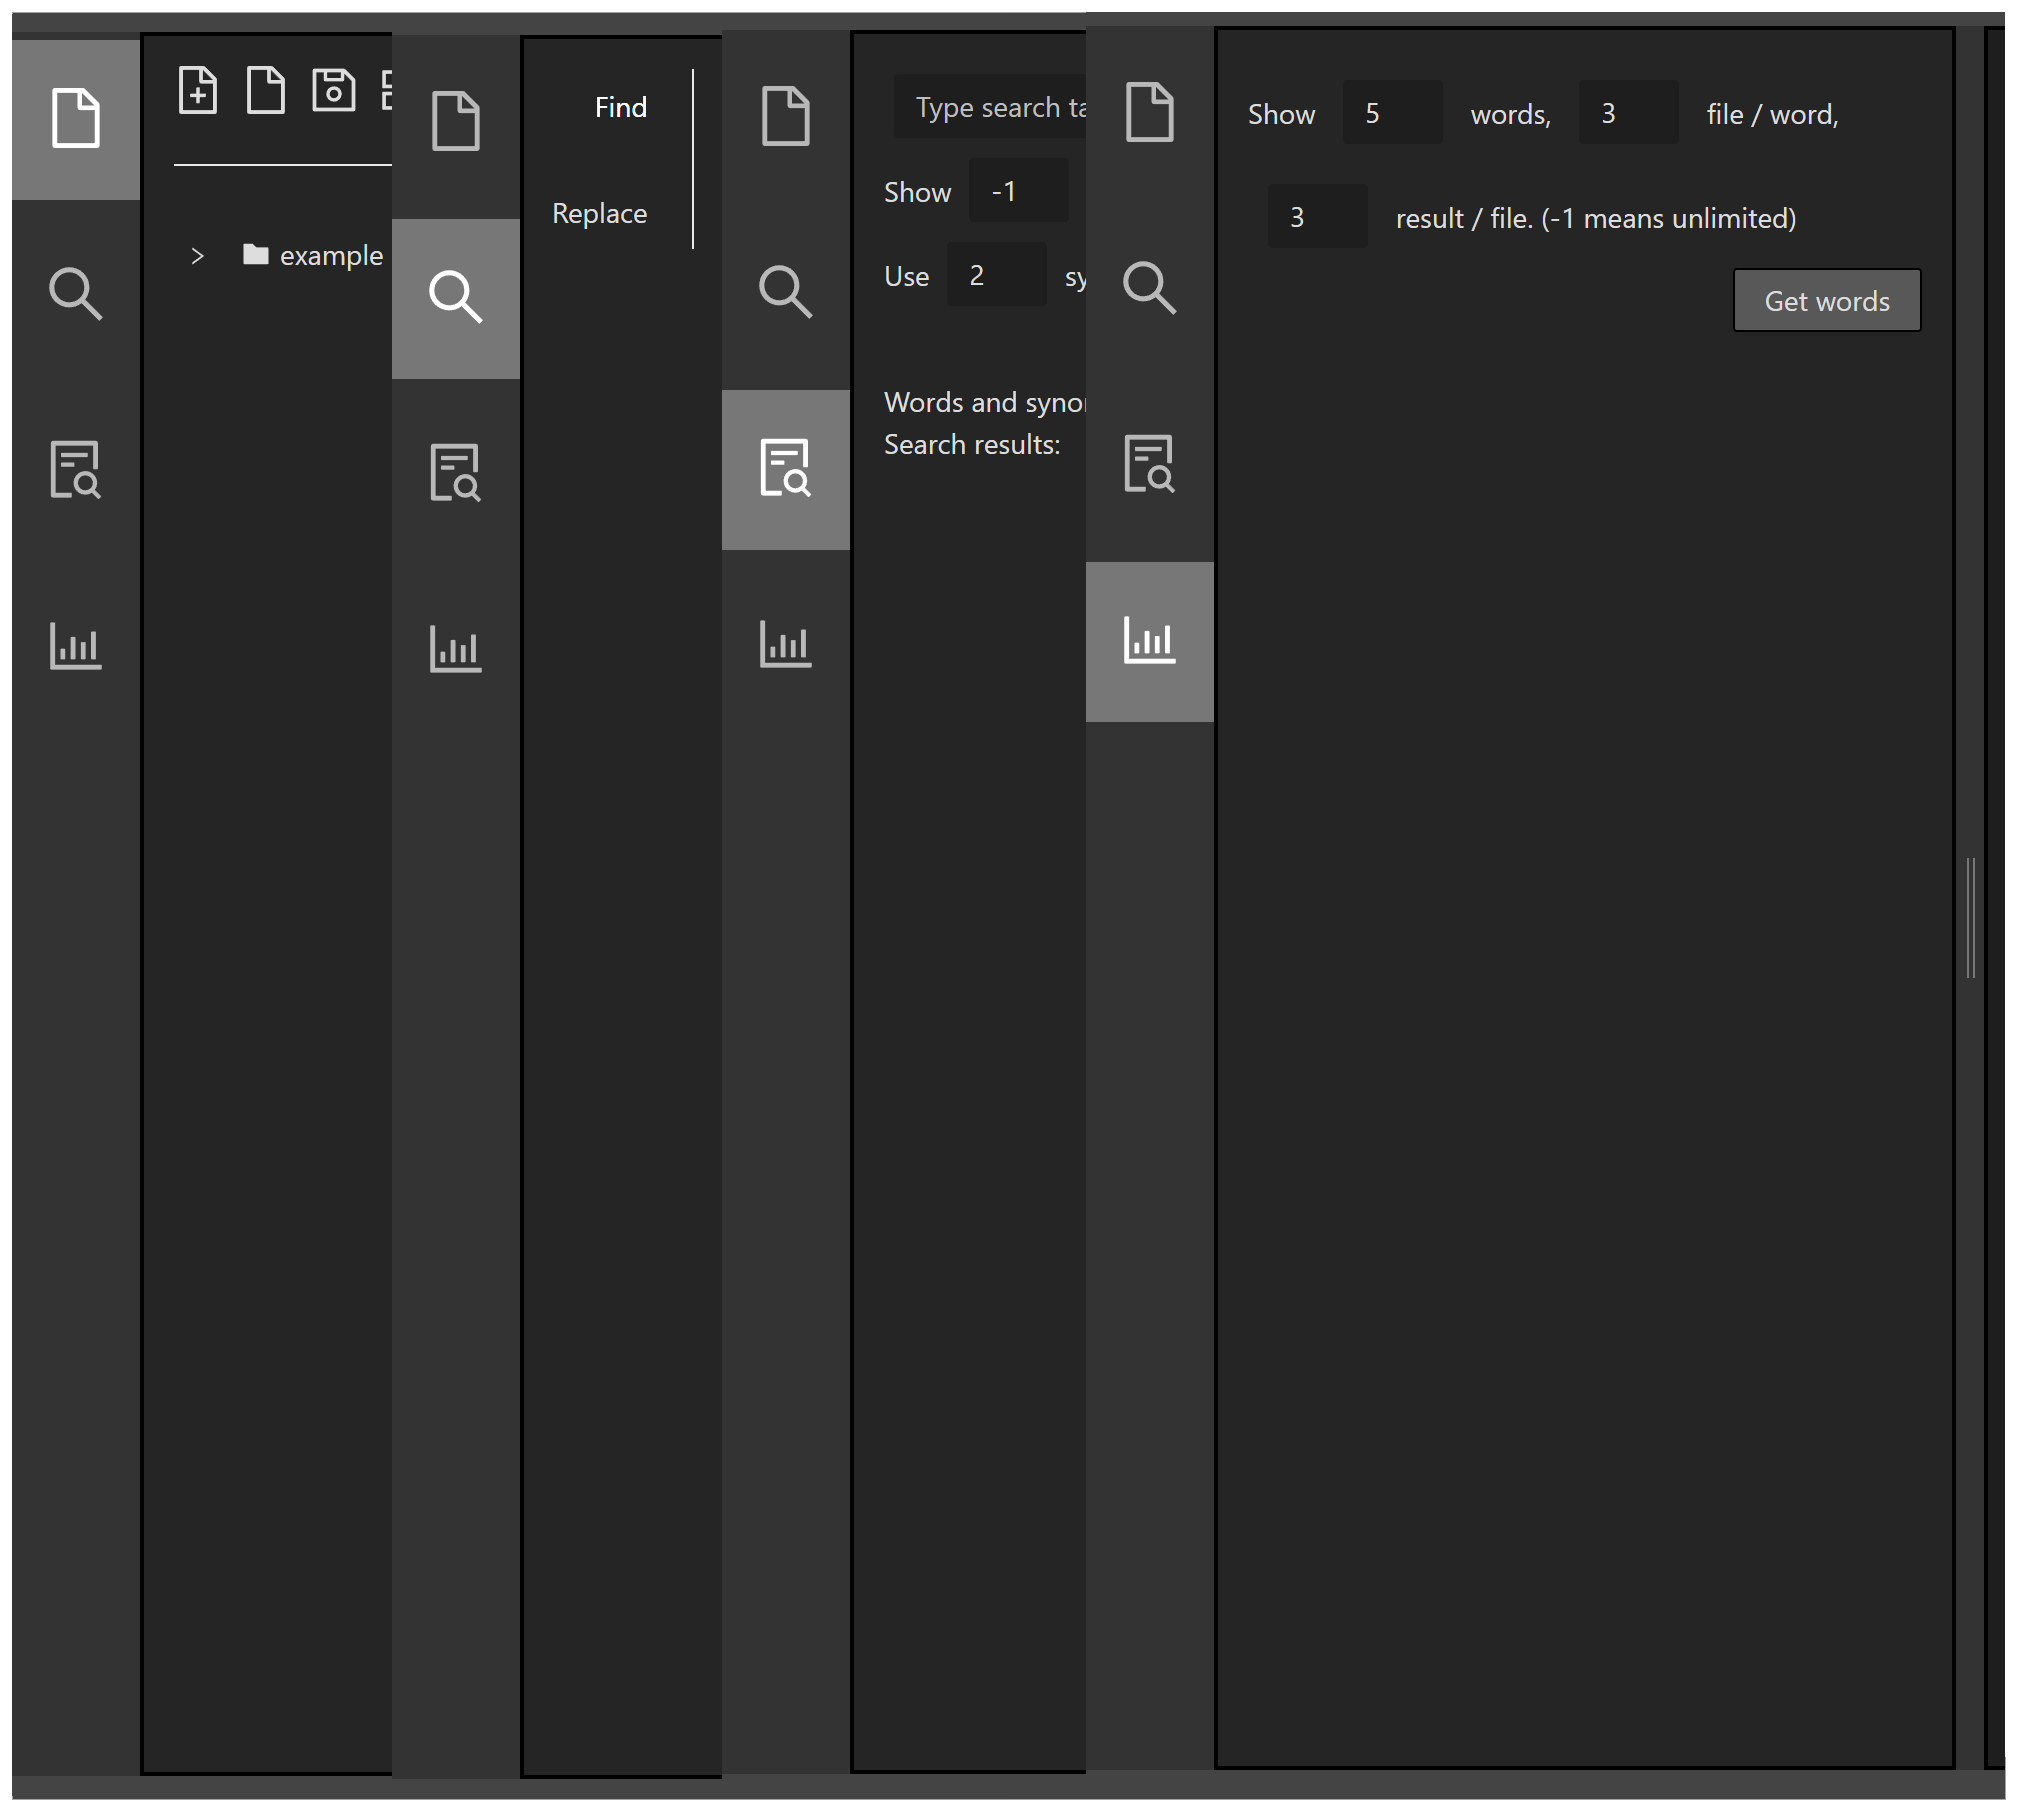
\includegraphics[width=0.6\textwidth]{images/dsacd-screenshot-sidebars.drawio.png}
    \caption{侧栏与菜单的选中高亮}
\end{figure}

\paragraph{编辑器栏部分}
编辑器栏部分的跳转模式类似金字塔模式和全连接模式的结合。其中开始界面类似金字塔模式中的“塔顶”,从这里可以重新选择工作区,而其他模块下可以回到这里。同时,另外三个模块又是全连接的,根据用户选中的文件、目录或未选中状态,自动进行任意切换。

在暂无内容提示和目录浏览器中,还会用很大号的文字提示用户当前所在状态,并且提示用户若要编辑文件应该怎么做。

\begin{figure}[h]
    \centering
    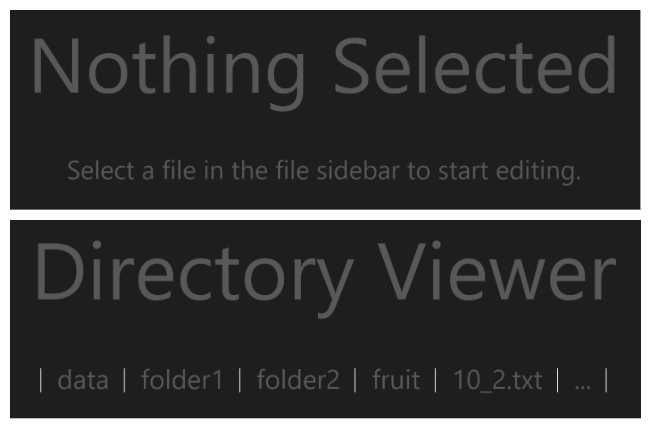
\includegraphics[width=0.6\textwidth]{images/dsacd-screenshot-editor-bar-hint.drawio.png}
    \caption{编辑器栏的提示}
\end{figure}

\subsection{形式层}

\paragraph{可收起标签侧栏}
系统整个侧栏采用标签模式和可收起面板的结合设计模式。侧栏可以选择标签,选中的侧栏会高亮;同时侧栏也可以选择收起。如下图中,展示了侧栏选择不同标签和收起的效果。

同时,鉴于侧栏和编辑器栏可以自由滑动,自定义两栏的空间分布,一定程度上实现了可移动面板的设计模式。

此外,菜单栏特意设计放在界面最左边,用户可以直接将鼠标移动到最左侧即可选择侧栏。

\begin{figure}[h]
    \centering
    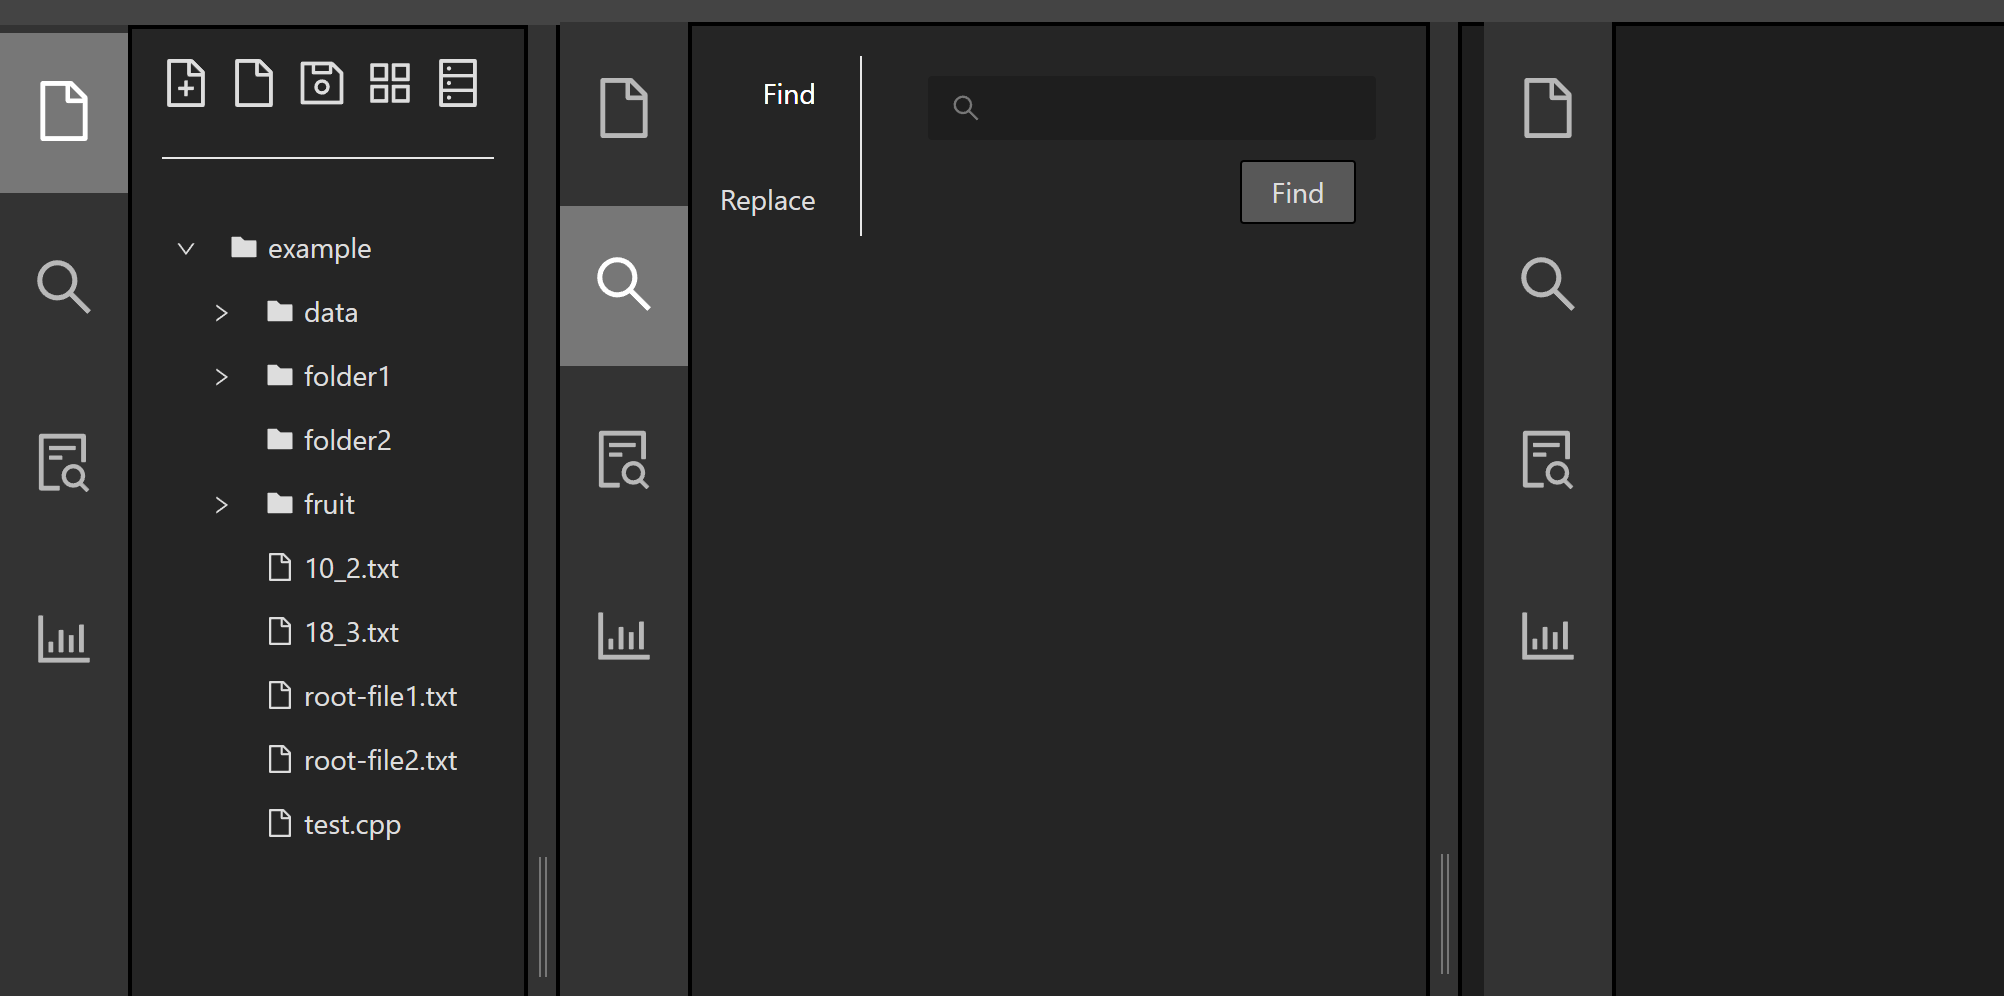
\includegraphics[width=\textwidth]{images/形式-可收起侧栏.png}
    \caption{可收起标签侧栏}
\end{figure}

\clearpage

\paragraph{编辑器栏位于中心舞台}
作为核心编辑区,编辑器栏位于整个界面的中心舞台。页眉、页脚、菜单栏和侧栏均围绕其周围。其中侧栏虽然可以调整和编辑器栏的占比,但最多不超过50\%,即侧栏占空间一定不会超过编辑器栏。

\begin{figure}[h]
    \centering
    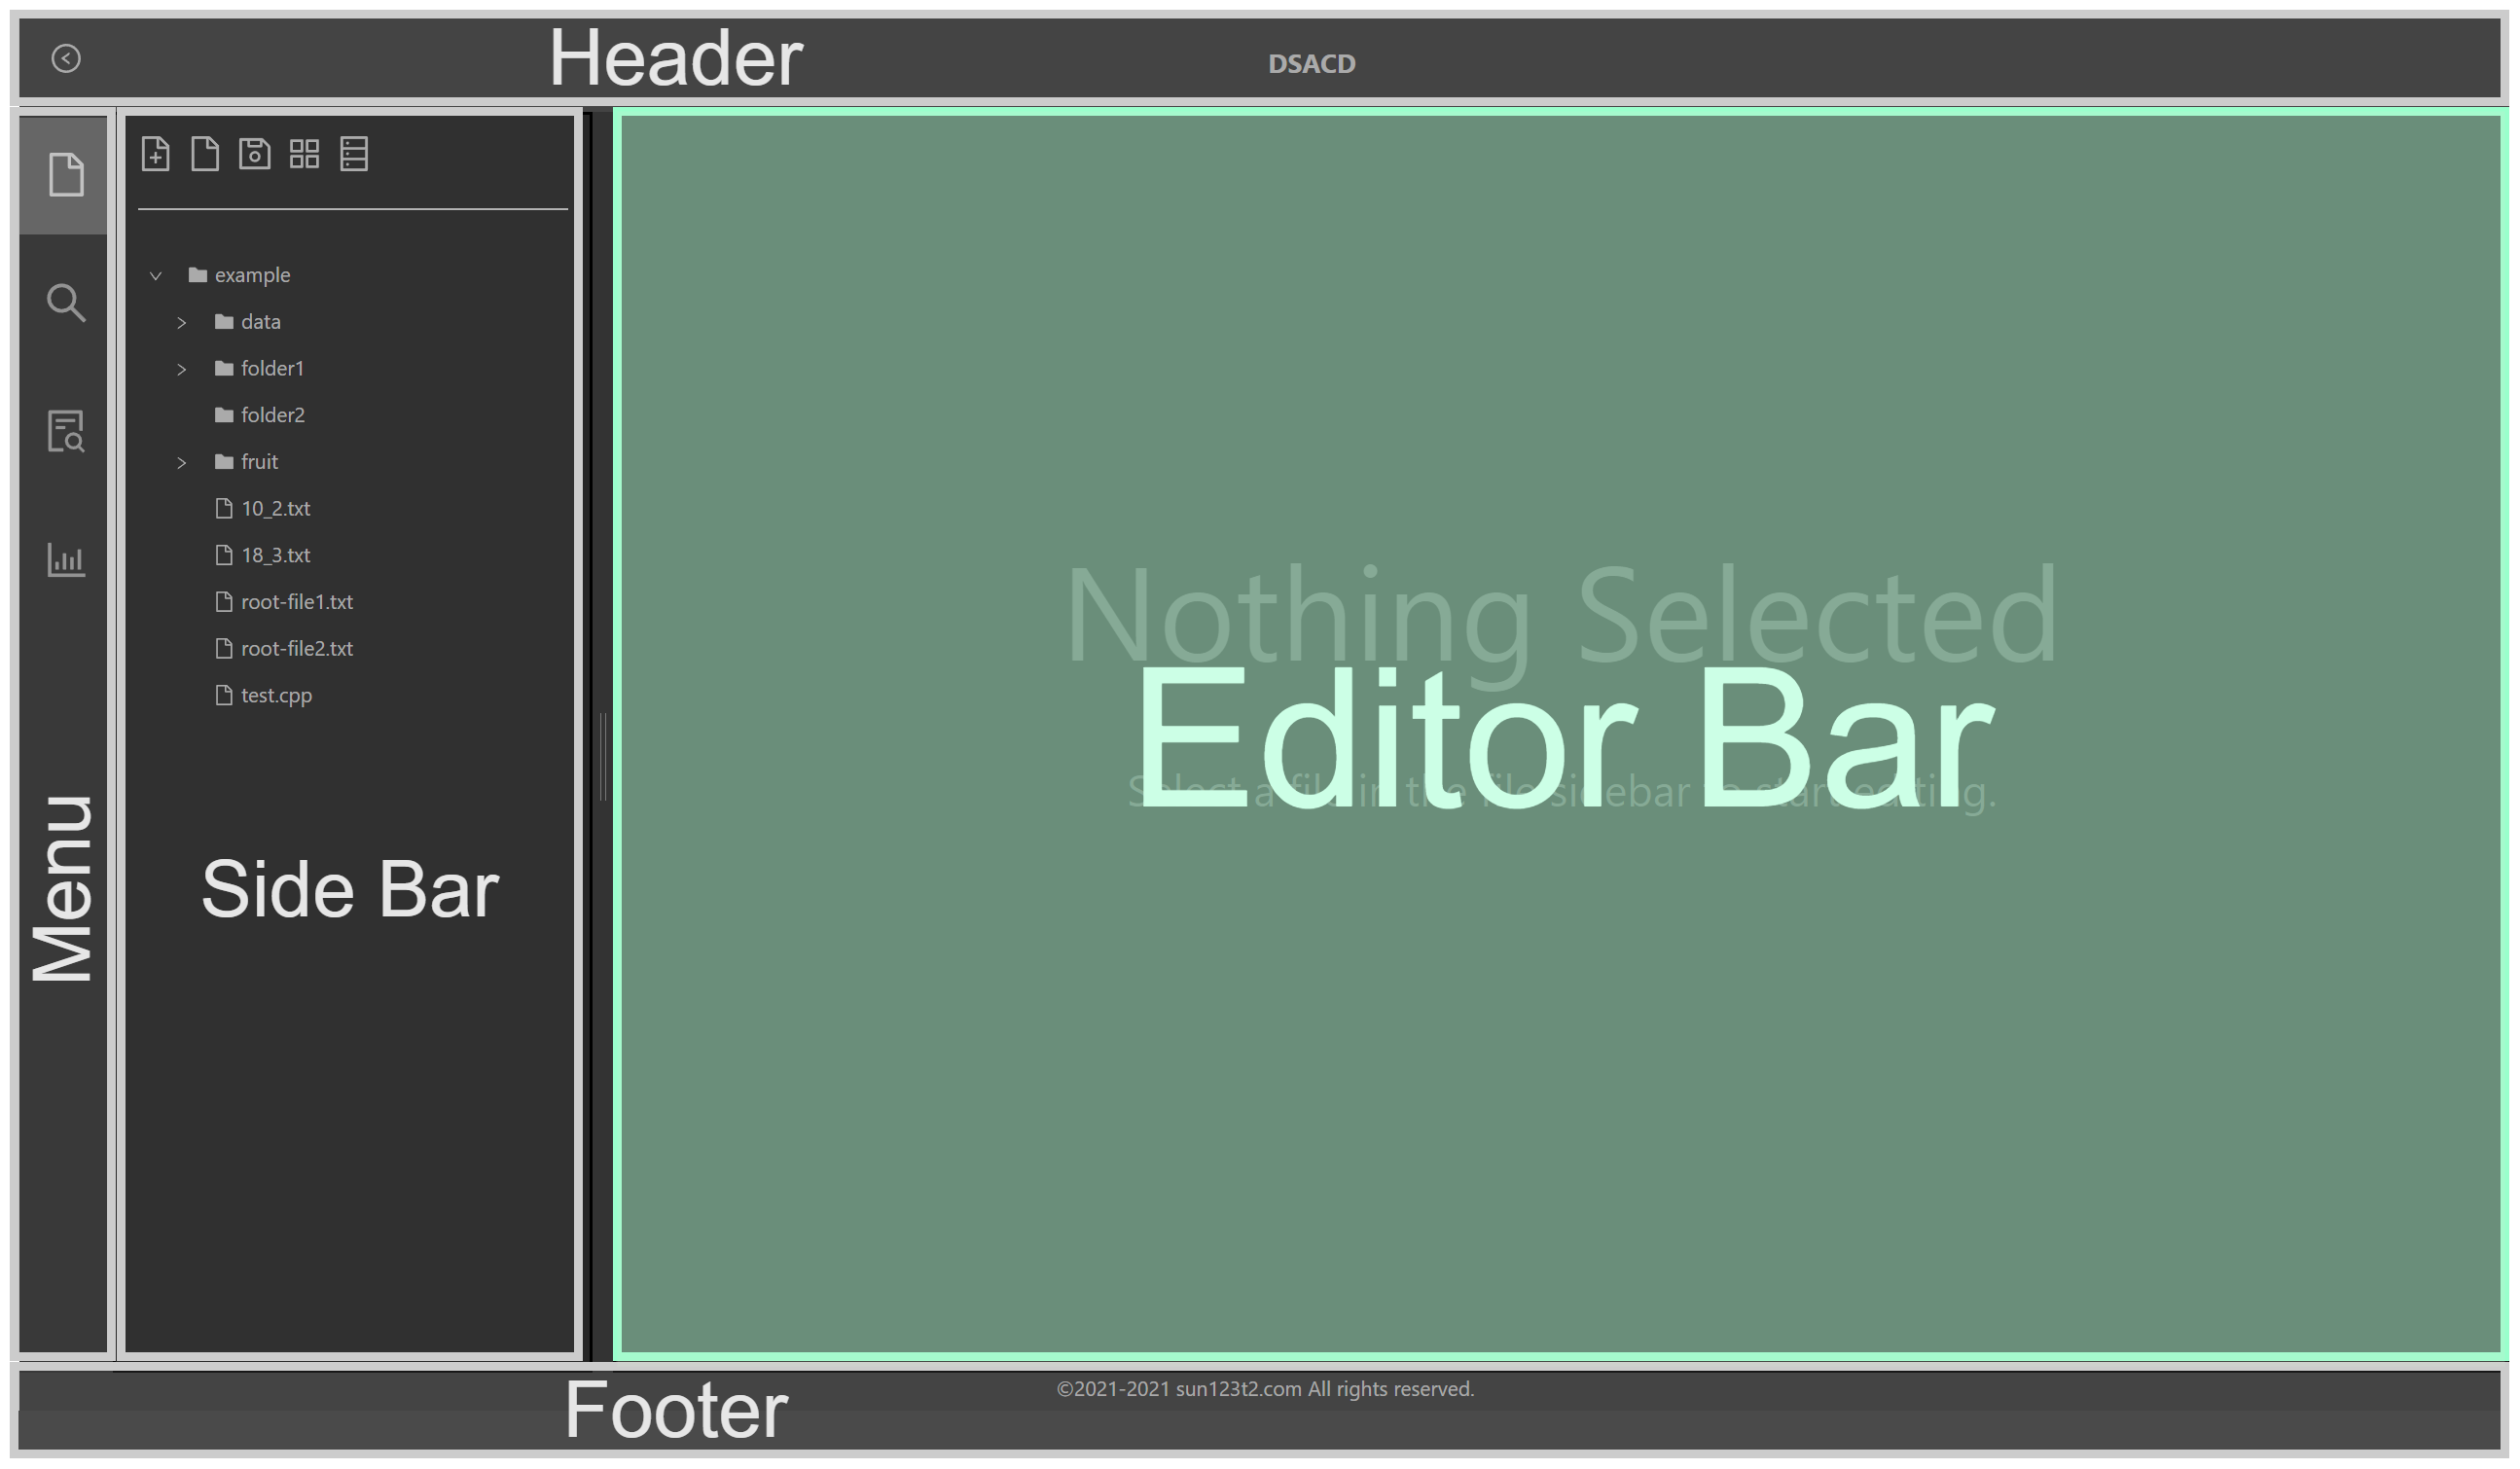
\includegraphics[width=0.8\textwidth]{images/dsacd-screenshot-center.drawio.png}
    \caption{编辑器栏位于中心舞台}
\end{figure}

\paragraph{手风琴方式显示结果}
多文件检索、词频统计的结果包含关键词、文件、匹配位置等多维度信息,需要多层次显示。这里设计采用手风琴的设计模式进行显示,用户可以收起或展开任意单元,重点查看自己关注的部分。(注:由于时间原因,二代原型中尚未实现此功能,待目标产品中得以实现)

此外,用户可以设置每个层次显示的数量,达到一下子可以查看自己期望数量的效果(如希望多看到几个文件、或希望看到前几个文件的多几项内容等)。

\begin{figure}[h]
    \centering
    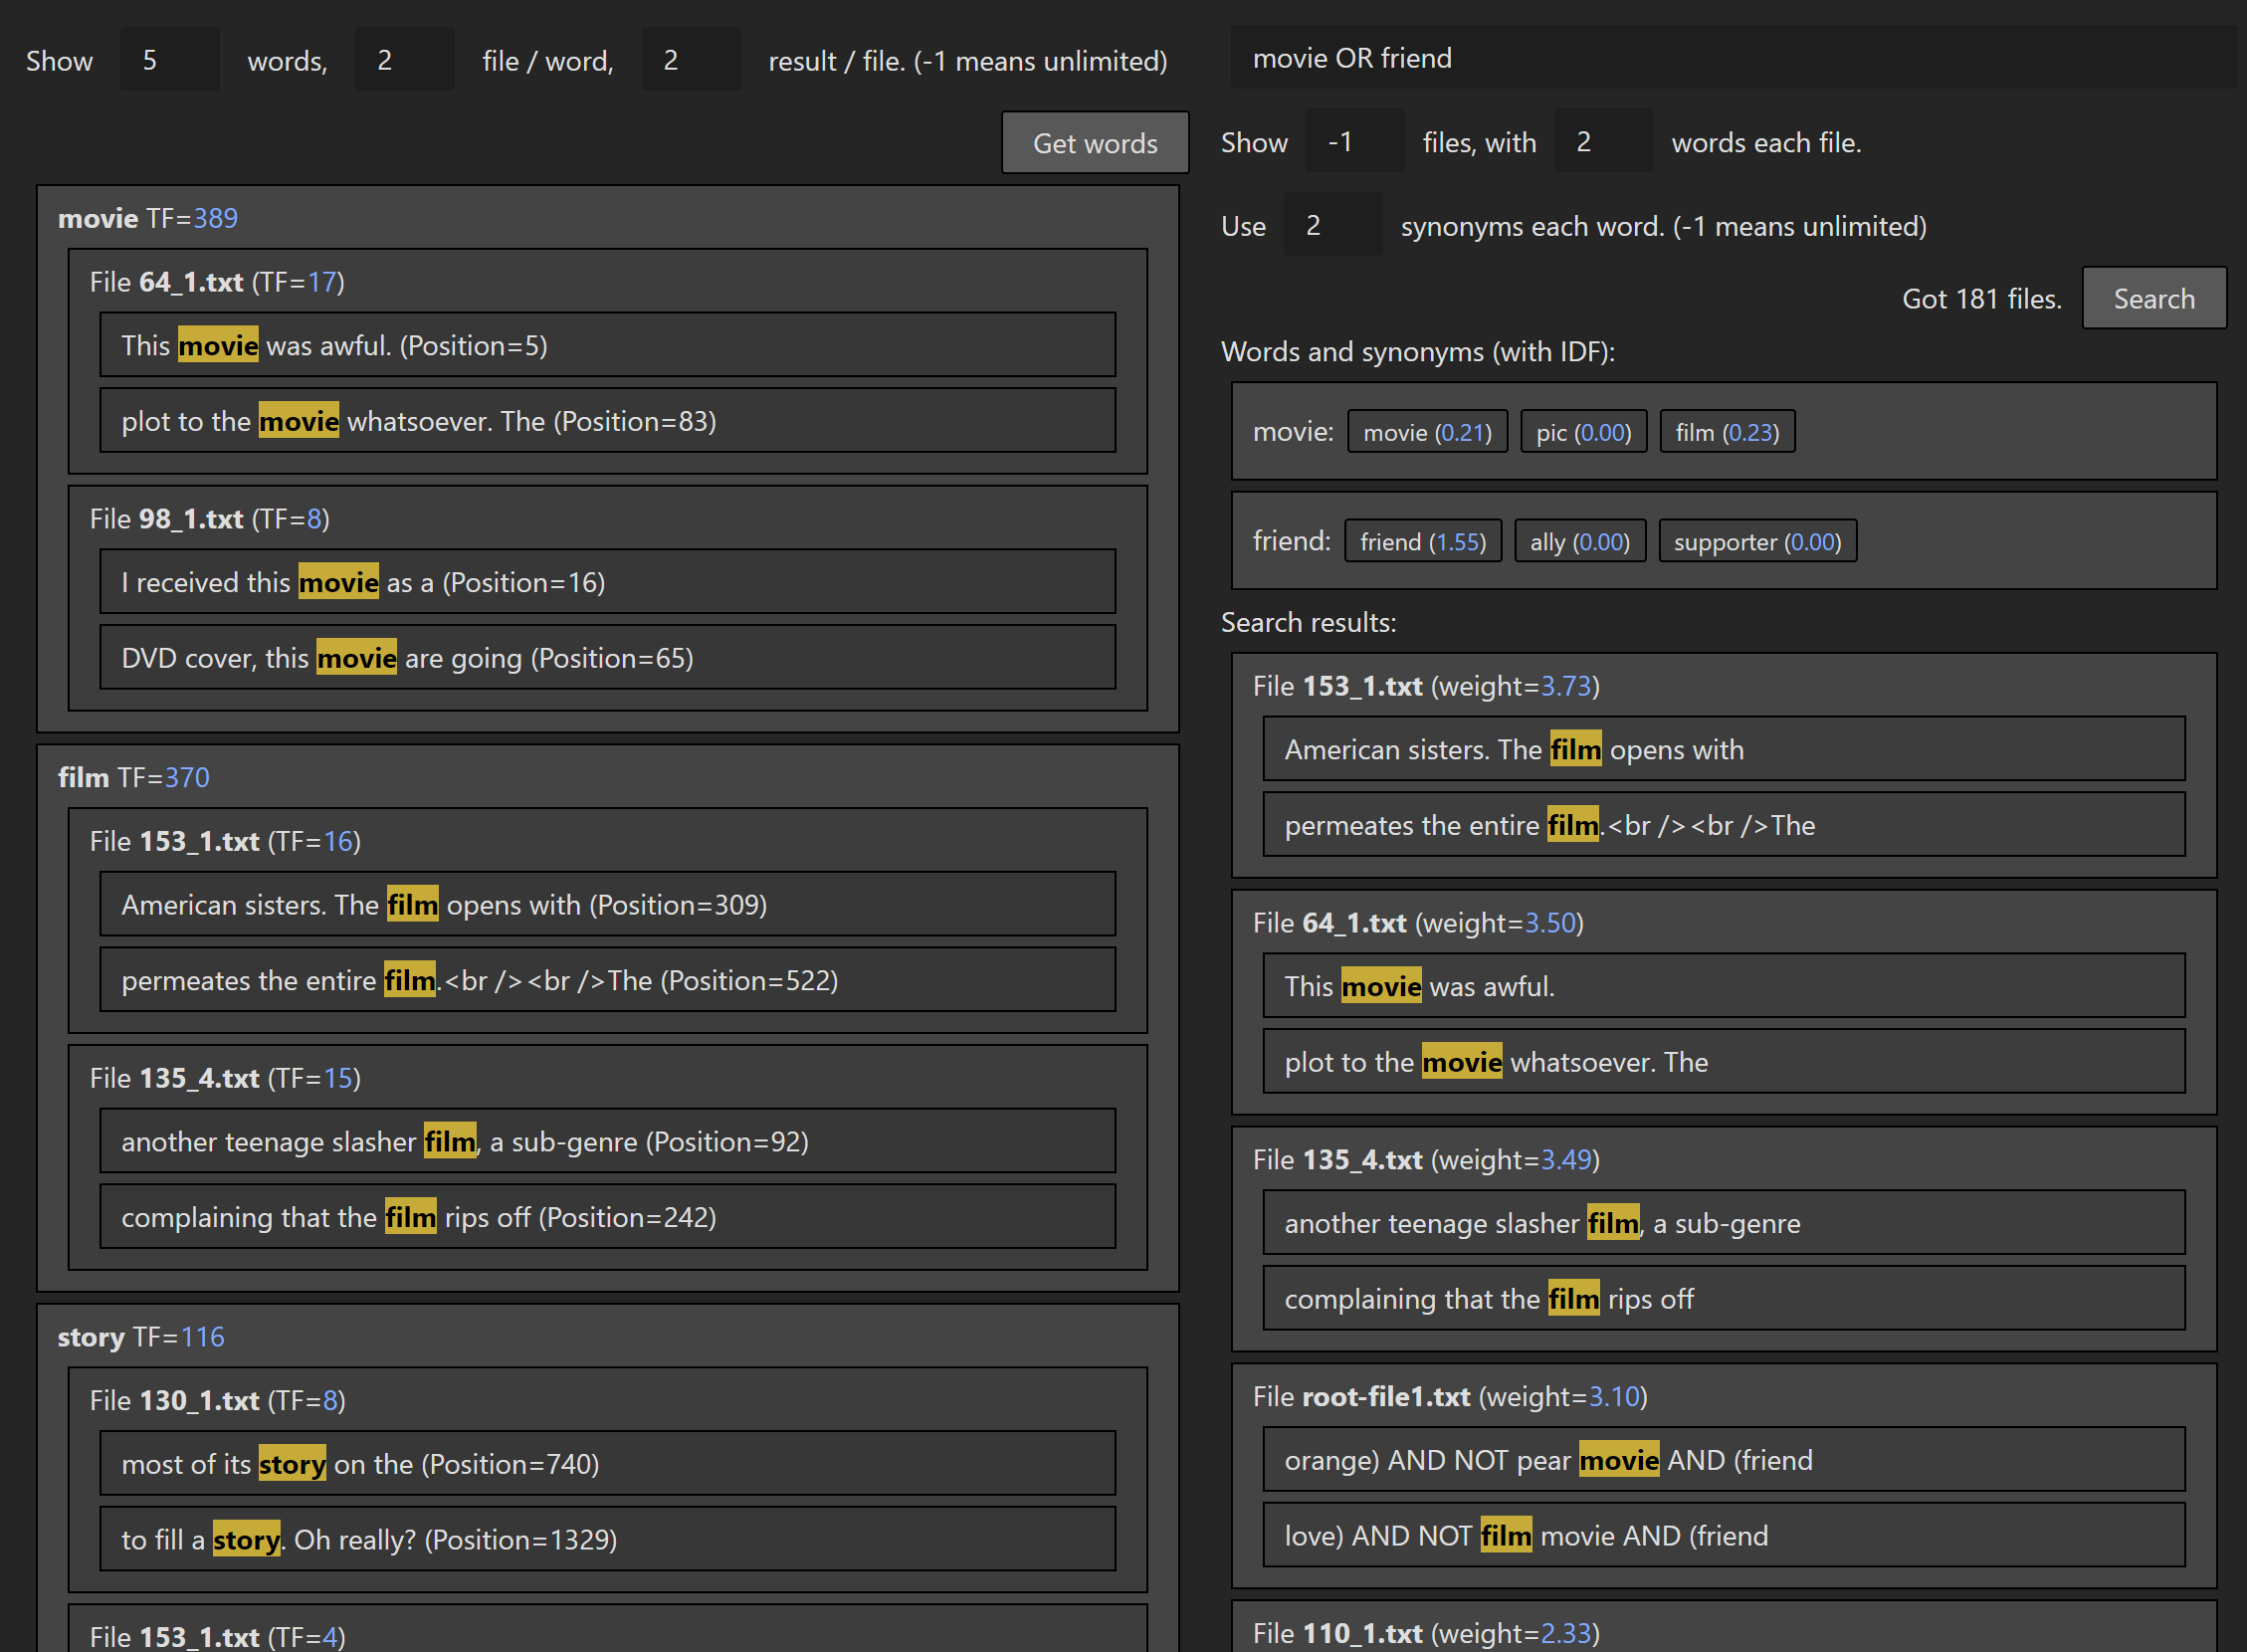
\includegraphics[width=0.8\textwidth]{images/形式-检索结果.png}
    \caption{手风琴方式显示结果}
\end{figure}

\clearpage

\paragraph{文件按钮对等网格}
文件管理侧栏中有五个地位相当的文件管理按钮,分别为:新建、打开、保存、全部保存、更新已保存信息。它们采用对等网格的方式,大小相当、间距相等地排为一排。

\begin{figure}[h]
    \centering
    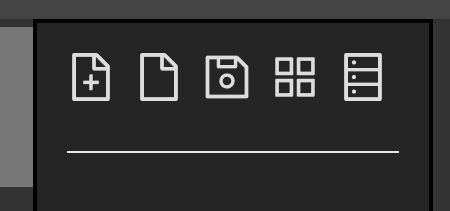
\includegraphics[width=0.4\textwidth]{images/形式-文件按钮.png}
    \caption{文件操作按钮}
\end{figure}

\paragraph{侧栏内部流式布局}
侧栏内部采用流式布局,以此保证在不同的侧栏宽度下都能获得较好的显示效果。下面以词频侧栏为例,可见在不同宽度下会自适应将内容以恰当的方式排版显示。

\begin{figure}[h]
    \centering
    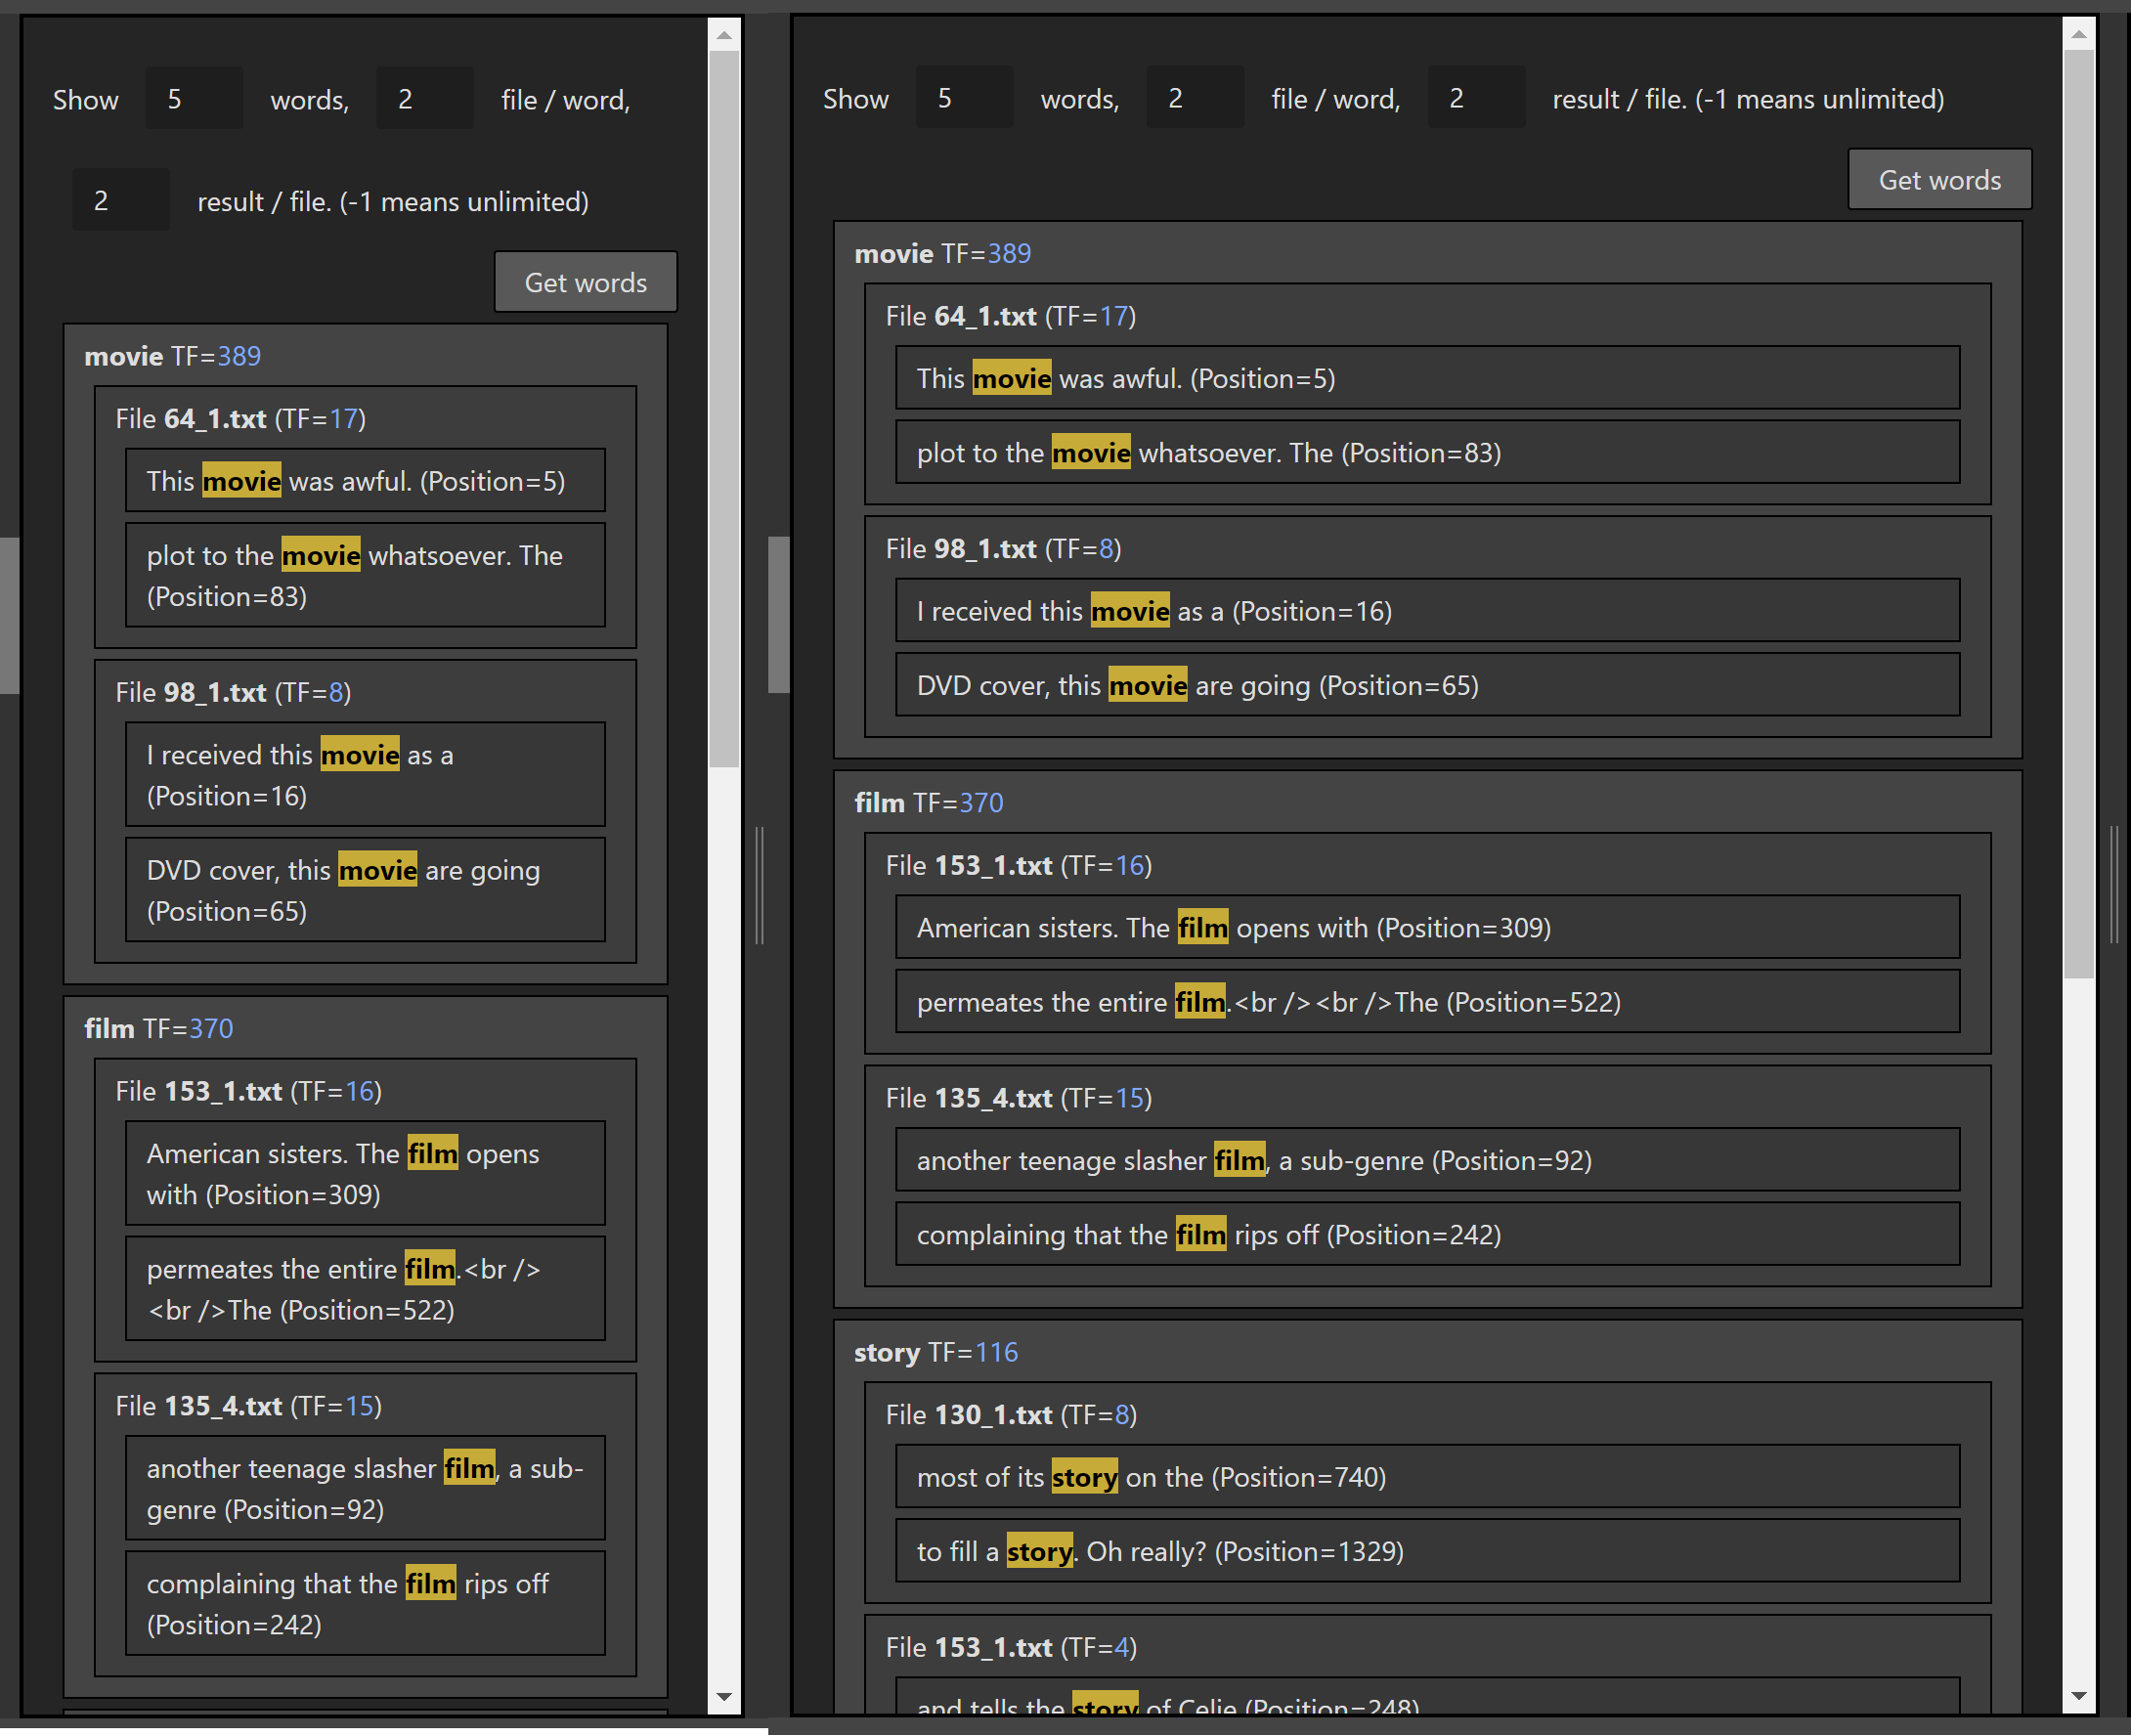
\includegraphics[width=\textwidth]{images/形式-流动.png}
    \caption{流式布局的侧栏}
\end{figure}

\clearpage

\subsection{细节层}

\paragraph{多选一或零}
系统中存在许多“多选一或零”的交互设计。具体而言,就是可以可以从多个目标中不选,或最多同时选择一个。

具体地说,选择任意一个未选中的选项,会切换至那个选择,而再次点击当前选中的选项会取消选择,什么也不选中。

这种设计应用于以下位置:
\begin{outline}
    \1 菜单栏的侧栏选择(在形式层中第一点已经说明)
    \1 文件树中选择文件或目录
    \1 检索替换侧栏中选择检索结果
\end{outline}

\begin{figure}[h]
    \centering
    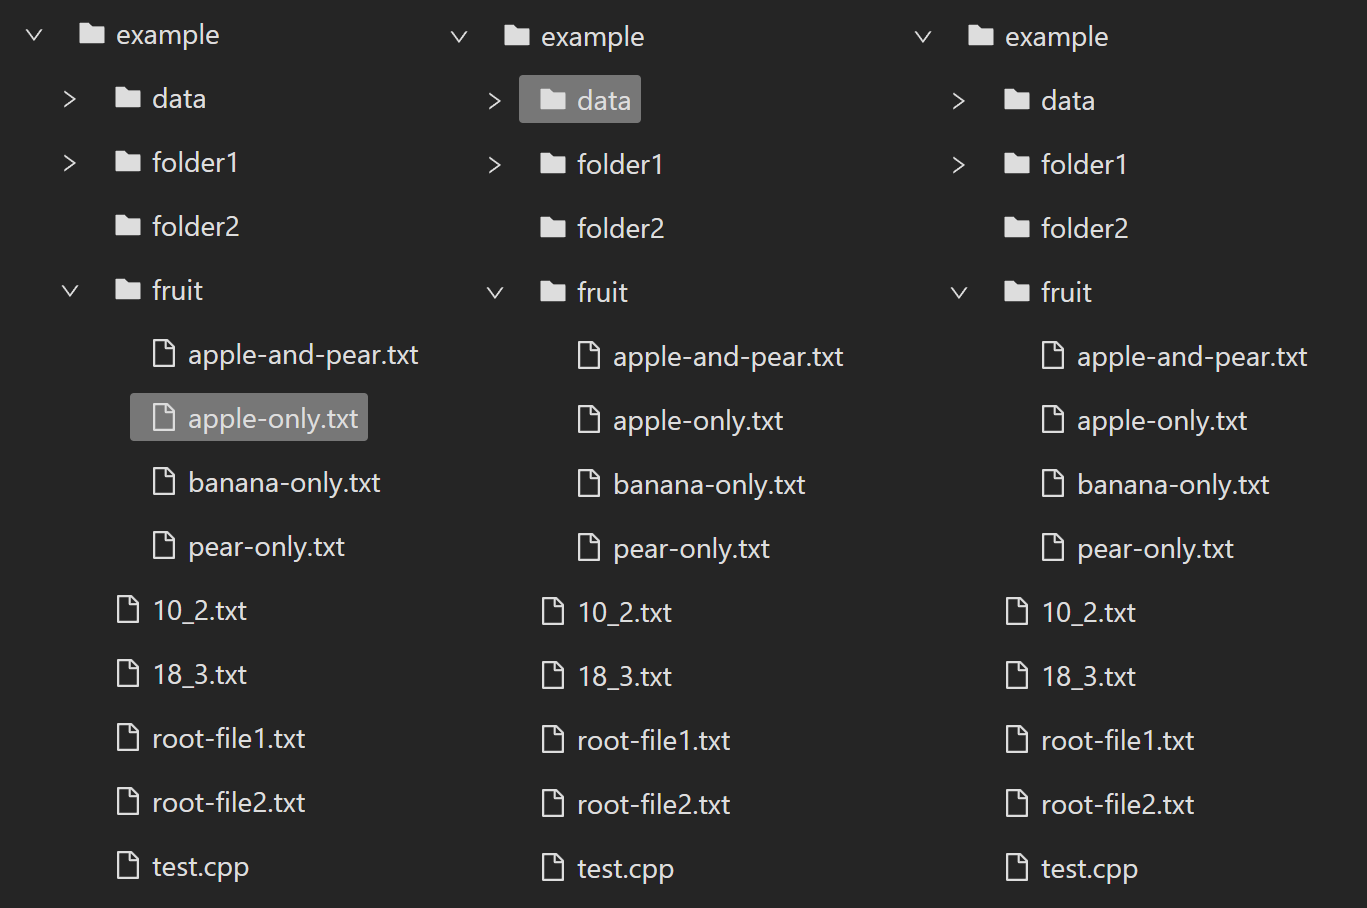
\includegraphics[width=0.8\textwidth]{images/细节-文件多选一或零.png}
    \caption{文件侧栏中的选择}
\end{figure}

\begin{figure}[h]
    \centering
    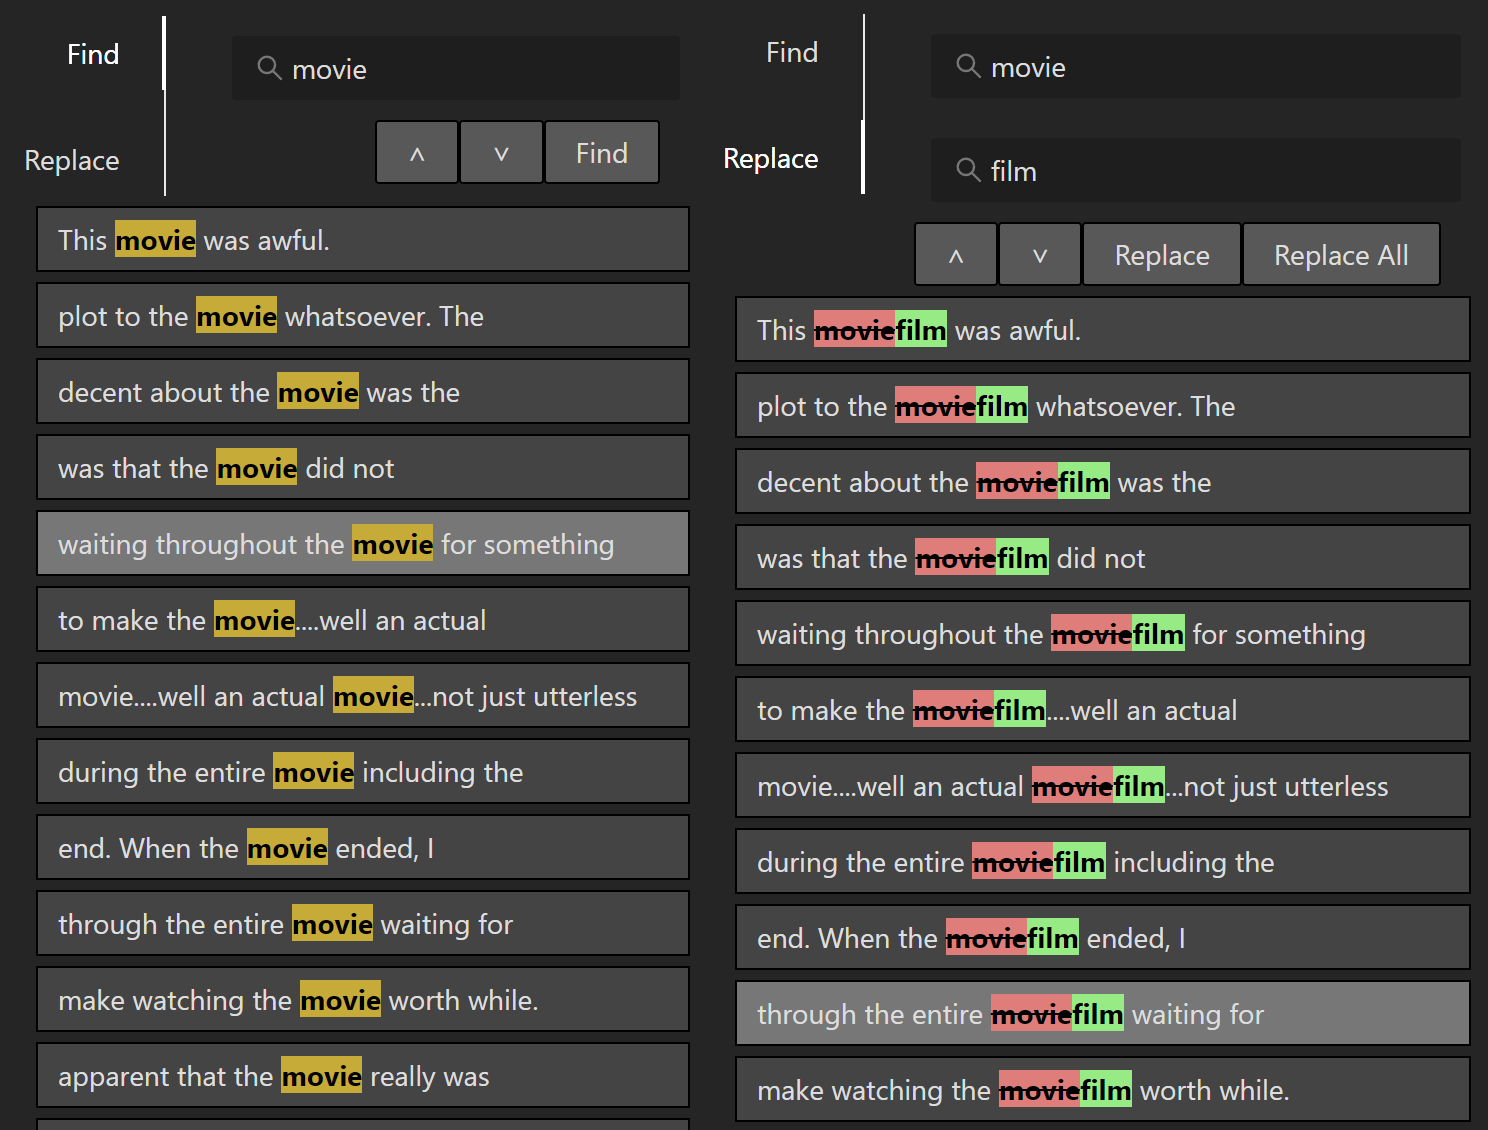
\includegraphics[width=0.7\textwidth]{images/细节-多选一.png}
    \caption{检索替换侧栏中的选择}
\end{figure}

\clearpage

\paragraph{内联文本输入提示}
在检索替换侧栏中,内联检索图标提示输入检索、替换内容。

\begin{figure}[h]
    \centering
    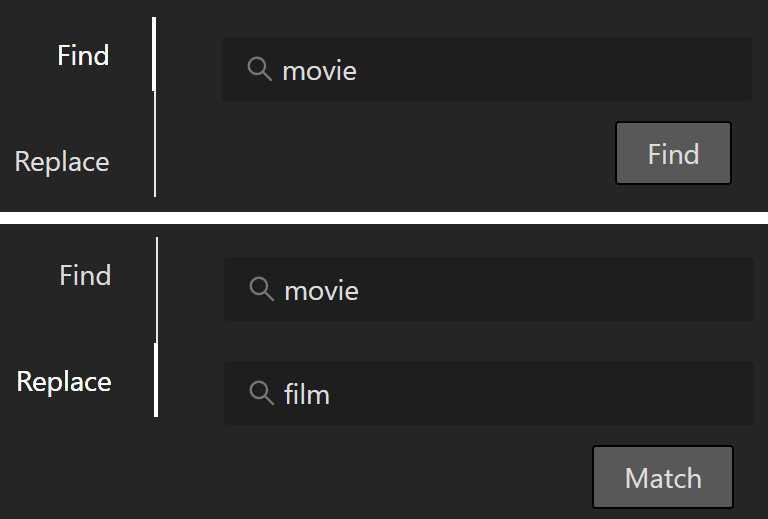
\includegraphics[width=0.6\textwidth]{images/细节-内联提示.png}
    \caption{内联的检索图标提示}
\end{figure}

\paragraph{填空输入}
在多文件检索和词频统计侧栏中,使用填空输入的方式自定义需要显示的条目和内容。

\begin{figure}[h]
    \centering
    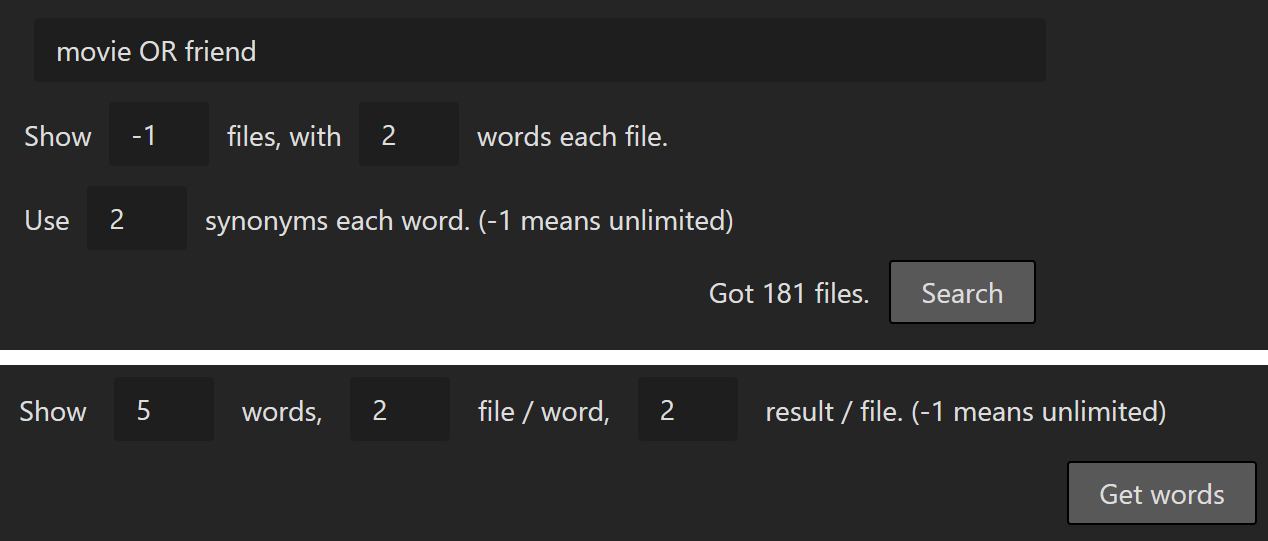
\includegraphics[width=0.8\textwidth]{images/细节-填空输入.png}
    \caption{内联的检索图标提示}
\end{figure}

\clearpage

\part{用户测试}

我用二代原型与邓栊涛同学进行了互测,他指出了原型中存在以下问题。我对反馈的问题进行了分类整理。

\section{问题汇总}

\subsection{逻辑问题}
\paragraph{单文件编辑模式}
应用场景中设想了单文件编辑、多文件检索两种模式,但二代原型设计中,开始界面的三个按钮都是针对文件夹进行操作的。这就类似只能对工程操作的IDE,即使只有一个文件也要新建工程,对于单文件编辑显得十分麻烦。

\begin{figure}[h]
    \centering
    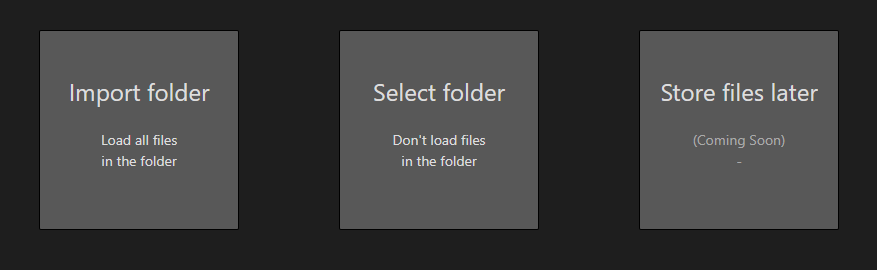
\includegraphics[width=0.8\textwidth]{images/问题-单文件编辑.png}
    \caption{开始界面的三个按钮}
\end{figure}

\subsection{习惯问题}
\paragraph{关闭当前文件}
二代原型设计中,关闭当前文件采用的是取消文件树中选中的方式。具体地说,就是打开某个文件时会在左侧高亮显示选中它,而再次点击高亮的部分即可关闭了。

但是邓同学反馈这样的方式与用户常规习惯不符,用户通常习惯于在上方点击“X”类似的按钮来关闭文件。

\begin{figure}[h]
    \centering
    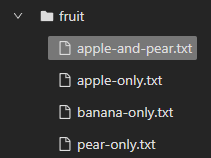
\includegraphics[width=0.4\textwidth]{images/问题-关闭当前文件.png}
    \caption{选中文件时高亮显示的效果}
\end{figure}

\clearpage

\subsection{说明缺失}
\paragraph{各侧栏的功能}
二代原型中采用最左侧的按钮对侧栏进行切换,每个按钮对应一个侧栏。每个按钮上有一个图标,但并没有文字说明其功能,为此用户可能不知道每个侧栏的功能是什么。

\begin{figure}[h]
    \centering
    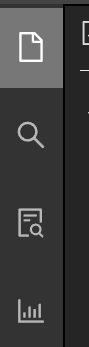
\includegraphics[width=0.1\textwidth]{images/问题-各侧栏功能.png}
    \caption{侧栏选择按钮}
\end{figure}

\paragraph{文件侧栏按键的功能}
文件侧栏中,有5个对文件进行操作的按钮,但同样是仅有图标而没有文字说明。

\begin{figure}[h]
    \centering
    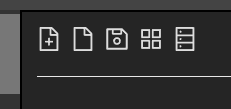
\includegraphics[width=0.4\textwidth]{images/问题-文件侧栏按钮.png}
    \caption{文件侧栏的五个按钮}
\end{figure}

\subsection{交互便利性}
\paragraph{数字输入框}
在多文件检索和词频统计侧栏中有许多自定义显示数量的数字输入框,但这些输入框没有输入限制和微调按钮,用户使用起来较不便利。

\begin{figure}[h]
    \centering
    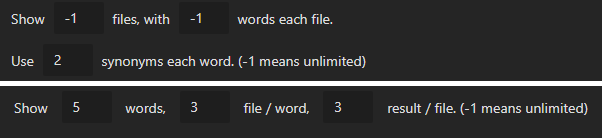
\includegraphics[width=\textwidth]{images/问题-数字输入框.png}
    \caption{多文件检索和词频统计侧栏的数字输入框}
\end{figure}

\clearpage

\paragraph{跳转不调整位置}
在检索替换、多文件检索和词频统计侧栏中,点击某个匹配项会自动跳转到对应文件,并选择匹配位置。但二代原型只会选中,而由于不确定用户右侧滚动条的位置,不保证用户右侧能看到选中的位置。

例如,下方配图中是较为边界的情况,用户只能看到选中词的一半。实际情况下许多时候整个词都看不到,需要用户手动滑动上下滚动条才能看到。

\begin{figure}[h]
    \centering
    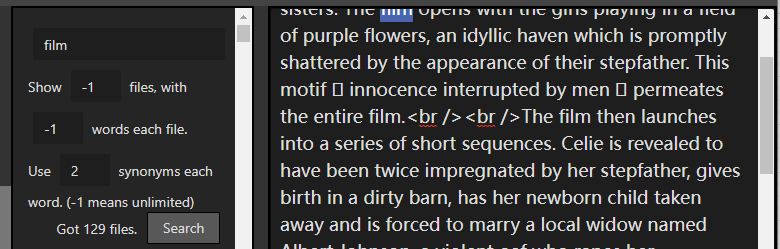
\includegraphics[width=0.8\textwidth]{images/问题-跳转不调整位置.png}
    \caption{多文件检索和词频统计侧栏的数字输入框}
\end{figure}

\paragraph{选中高亮背景色}
右侧文本编辑栏中选中时高亮的背景色为显眼的蓝色,但左边侧栏中选中时使用纯黑色高亮。这种高亮背景色很不明显,让用户难以分别选中和未选择的区域。

\begin{figure}[h]
    \centering
    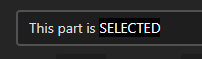
\includegraphics[width=0.4\textwidth]{images/问题-选中高亮背景色.png}
    \caption{侧栏选中高亮的效果}
\end{figure}

\clearpage

\part{改进说明}

经过用户测试后,部分问题在二代原型的基础上得到改进,结果为三代原型;而其余问题,由于技术和时间原因等待在目标产品中再进行改进,这里只说明改进的思路。

\section{三代原型中的改进}
\paragraph{关闭当前文件}
打开任意文件或目录时,标题旁添加了“X”符号,点击后即可关闭当前文件。这样的位置更符合用户关闭文件的习惯。

\begin{figure}[h]
    \centering
    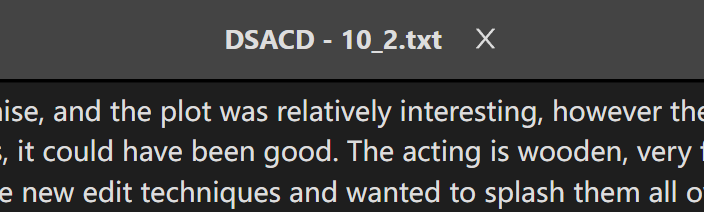
\includegraphics[width=0.6\textwidth]{images/改进-关闭文件.png}
    \caption{标题和旁边的关闭文件图标}
\end{figure}

\paragraph{功能说明}
二代原型中缺少说明的侧栏选择按钮、文件侧栏按钮,均在三代原型中添加了功能说明。将鼠标移动到图标上即会显示对应的说明。

\begin{figure}[h]
    \centering
    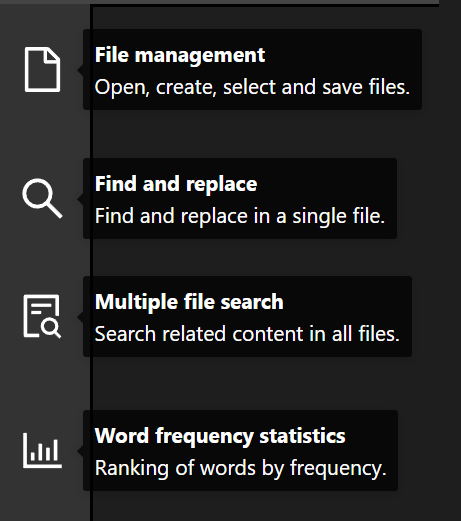
\includegraphics[width=0.4\textwidth]{images/改进-标签提示.png}
    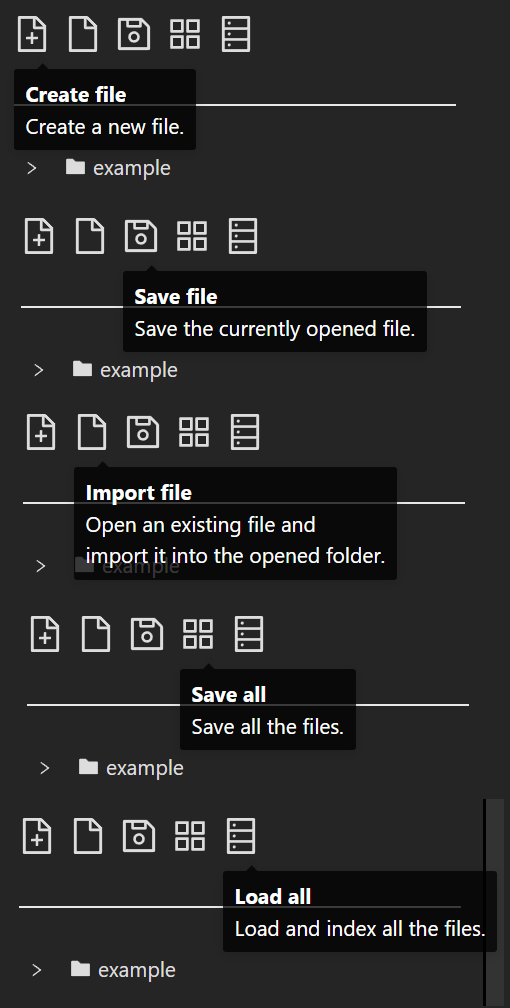
\includegraphics[width=0.4\textwidth]{images/改进-文件按钮提示.png}
    \caption{改进后的功能说明提示}
\end{figure}

\paragraph{数字输入框}
二代原型中的数字输入框没有任何限制,会在输入非法内容后报错。而三代原型中增加了输入的限制,同时附加了微调按钮(鼠标移动上去时会自动显示,其他时候隐藏)。

\begin{figure}[h]
    \centering
    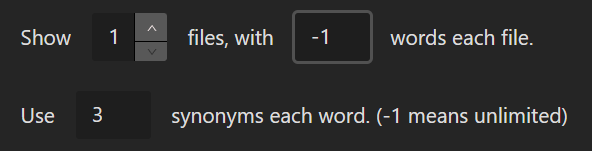
\includegraphics[width=0.6\textwidth]{images/改进-数字输入.png}
    \caption{改进后的数字输入框}
\end{figure}

\paragraph{高亮背景色}
任何地方选中时的背景色都被更正为了显眼的蓝色,可以方便用户明确选中的部分。

\begin{figure}[h]
    \centering
    
\includegraphics[width=0.4\textwidth]{images/改进-选中背景色.png}
    \caption{改进后的选中背景色}
\end{figure}

\section{待目标产品中的改进}
\paragraph{单文件编辑模式}
我在开始界面中新增了两个用于进入单文件编辑模式的按钮。但具体功能由于工作量较大,在三代原型中没有实现,待目标产品中得以实现。三代原型中点击它们会反馈特性尚未开发。

\begin{figure}[h]
    \centering
    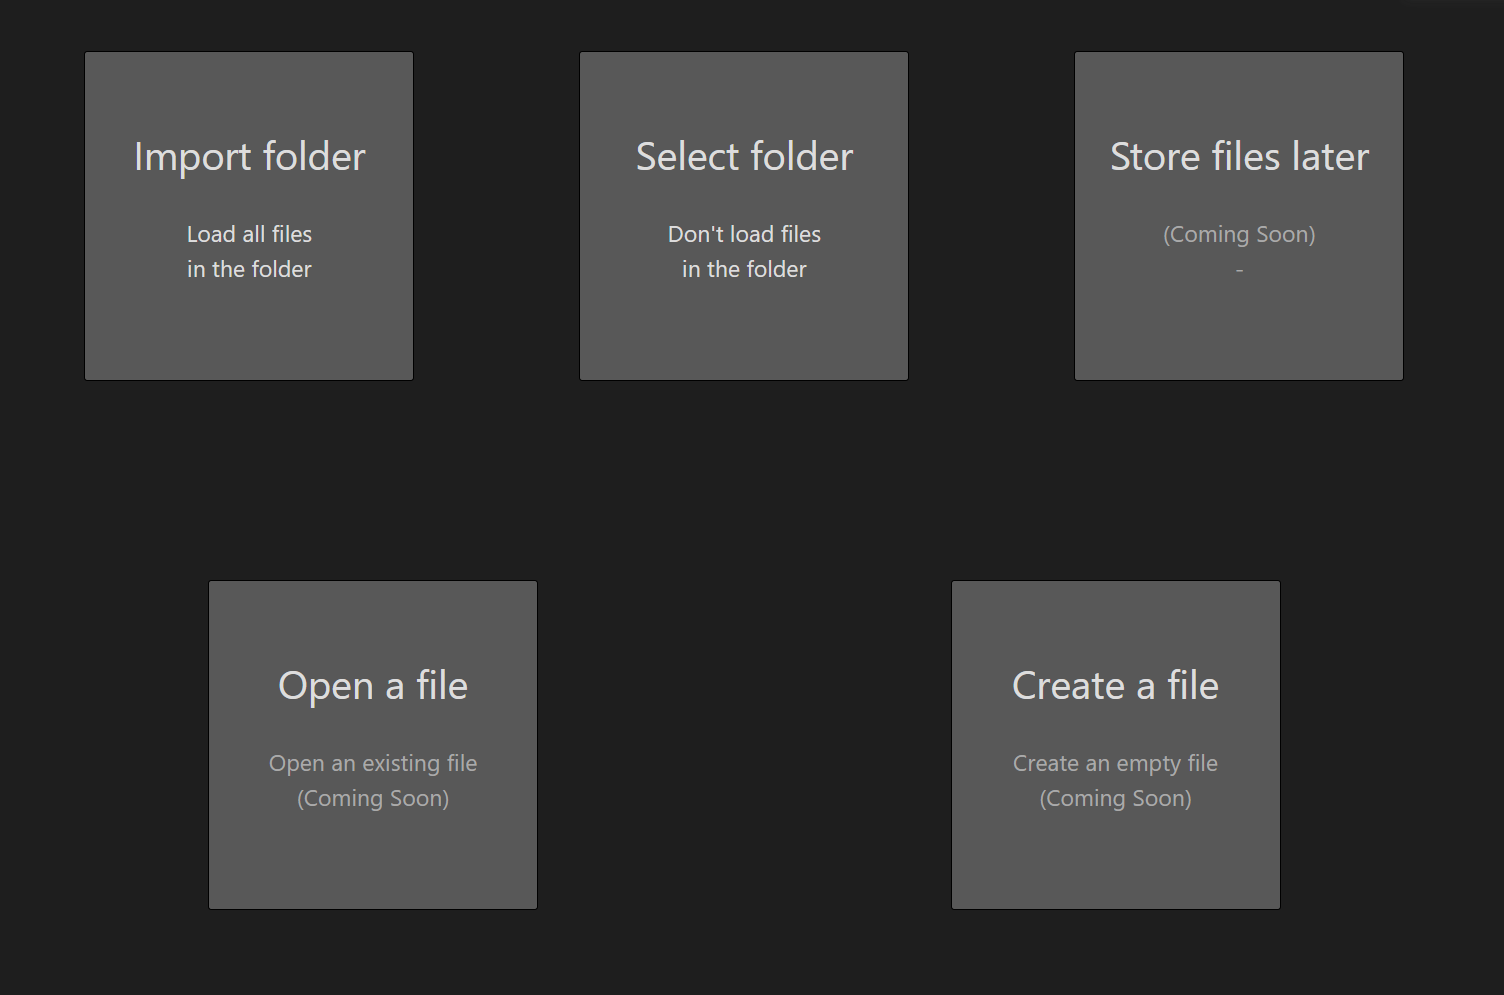
\includegraphics[width=0.6\textwidth]{images/改进-单文件编辑模式.png}
    \caption{单文件编辑模式的进入按钮}
\end{figure}

\paragraph{跳转不调整位置}
比较遗憾的是,这个需求虽然获取到了,我也很明确改进的思路。但是由于技术和时间的原因,无法在三代原型中改进。期待它在目标产品中得以实现。

\clearpage

\part{额外说明}

\section{关于数据结构课设}
此大作业复用了之前开发的数据结构课设,但我还是感到自己实践和改进了许多人机交互的设计。

\paragraph{两份工作集中在一个项目}
数据结构课设和人机交互的考核重点是不同的,这点从两个课程的报告中就能明显地看出来。
此报告中提到的交互设计在数据结构课设的报告中是只字未提的;同样地,数据结构和算法的设计在这里也只字未提。

因此,我不禁感觉到这两个方面较好地分割了我在这个文本编辑检索工具上完成的工作。在人机交互、数据结构与算法两方面我都尽全力去完成了,没有进行偷工减料,而二者又相得益彰,实现了$1+1>2$的效果,整体上实现了一个完成度较高的项目。我对这种工作的组合感到十分开心,希望之后能有更多机会实现这样的效果。

\paragraph{从发现到改进}
在仅以数据结构课设为目的进行设计和开发的过程中,其实我就已经实现了许多考虑人机交互的设计,但直到我学习了人机交互的知识我才发现。我想这主要由于两个方面:

\begin{outline}
    \1 整体设计照搬自VS Code,其中许多良好的设计也得到了继承
    \1 我在设计初期就考虑了用户实际使用的流程和体验,使得操作整体较为合理
    \1 之前使用软件的经验让我多少学习到了一些人机交互的模式,但我并不知道它们的名字,并且没有意识去主动使用
\end{outline}

二代原型中的人机交互设计有许多是“发现”的过程,让我重新认识了之前照搬或无意识实现的人机交互设计;而三代原型中的人机交互设计是我在重新思考和用户测试结合下,对系统进行改进得到的,主要是“改进”的过程。这两个过程都让我收获颇丰。

总而言之,虽然此大作业复用了数据结构课设,但人机交互设计的部分并没有偷工减料,经过“发现”和“改进”两个过程,让我对课上学到了知识有了更为深刻的认识。

\section{关于展示}
就我个人的角度,我认可自己完成的这份大作业。它还有很多值得改进的地方,但至少达成了我对于自己目前水平的期望。因此\textbf{如果老师也认可我的大作业值得与同学们分享,我希望将这个项目分享给同学们},谢谢老师。

\section{鸣谢}

\paragraph{指导教师:李童老师}
首先,要感谢李童老师对我们细致而透彻的讲解、以及耐心地回答我下课提出的问题。十分感谢老师的教导,让我对之前使用软件和开发软件中用到的人机交互设计。此外,我本次大作业中改进的部分,也让我加深了对人机交互设计模式的理解。

\paragraph{分组互测:邓栊涛同学}
与我互测的邓同学同样对此大作业帮助很大,用户测试的反馈意见对改进软件十分珍贵。邓同学的反馈意见让我意识到了之前设计中的不足之初,启示了我从更加真实的用户的角度思考这个项目。邓同学十分耐心地提出了十余条意见,符合人机交互的准则,且考虑细致周到。

\paragraph{iStar模型知识:王云铎学长}
王云铎学长有一次组织的用户访谈,调查开发者使用iStar模型进行需求分析的感受。而我有幸称为了其中的被试之一。这次参与让我学会了iStar基础的表示方法,也对需求工程有了一定的了解。此大作业需求分析中使用的iStar模型也多亏了之前参与那次访谈学习到的知识。为此,十分感谢云铎学长。

注:这里鸣谢两位同学的顺序不分先后,不具有贡献大小关系的含义。

\end{document}